\documentclass[xcolor={x11names}, aspectratio=169 ]{beamer}

\usepackage{tikz}
\usepackage{pgfplots}
\pgfplotsset{compat=1.16}

\usepackage{colortbl}
\usetikzlibrary{positioning,plotmarks}

\usepackage{graphicx}
\usepackage{hyperref}
\usepackage{mathtools}
\usepackage{amssymb}
\usepackage{tcolorbox}
\usepackage{multirow}
\DeclareMathOperator*{\argmax}{arg\,max}
\usepackage{booktabs}

\usetikzlibrary{arrows.meta, positioning, patterns, calc, shapes, shapes.geometric, decorations.pathreplacing, quotes, backgrounds, fit}

% Theme settings
\usetheme{Madrid}
\usecolortheme{seahorse}
\setbeamertemplate{navigation symbols}{}

% ============================================
% SECTION NAVIGATION SETUP
% ============================================
% Show current section in headline
\setbeamertemplate{headline}{%
  \leavevmode%
  \hbox{%
    \begin{beamercolorbox}[wd=\paperwidth,ht=2.5ex,dp=1.125ex]{palette quaternary}%
      \insertsectionnavigationhorizontal{\paperwidth}{}{\hskip0pt plus1filll}
    \end{beamercolorbox}%
  }
}

% Add footline with current part/section info
\setbeamertemplate{footline}{%
  \leavevmode%
  \hbox{%
    \begin{beamercolorbox}[wd=.333333\paperwidth,ht=2.25ex,dp=1ex,center]{author in head/foot}%
      \usebeamerfont{author in head/foot}\insertshortauthor
    \end{beamercolorbox}%
    \begin{beamercolorbox}[wd=.333333\paperwidth,ht=2.25ex,dp=1ex,center]{title in head/foot}%
      \usebeamerfont{title in head/foot}\insertshorttitle
    \end{beamercolorbox}%
    \begin{beamercolorbox}[wd=.333333\paperwidth,ht=2.25ex,dp=1ex,right]{date in head/foot}%
      \usebeamerfont{date in head/foot}\insertframenumber{} / \inserttotalframenumber\hspace*{2ex}
    \end{beamercolorbox}%
  }%
  \vskip0pt%
}

% Custom commands
\newcommand{\E}{\mathbb{E}}

% ============================================
% PROOF BOX ENVIRONMENT (Grey)
% ============================================
\newtcolorbox{proofbox}[1][]{
    colback=gray!15,
    colframe=gray!50,
    boxrule=1pt,
    arc=3pt,
    left=6pt,
    right=6pt,
    top=6pt,
    bottom=6pt,
    fonttitle=\bfseries,
    title={#1}
}

% Section transition slide command
\newcommand{\sectionslide}{%
  \begin{frame}
    \vfill
    \centering
    \begin{beamercolorbox}[sep=8pt,center,shadow=true,rounded=true]{title}
      \usebeamerfont{title}\insertsectionhead\par%
    \end{beamercolorbox}
    \vfill
  \end{frame}
}

% Part transition slide command
\newcommand{\partslide}{%
  \begin{frame}
    \vfill
    \centering
    \begin{beamercolorbox}[sep=12pt,center,shadow=true,rounded=true]{palette primary}
      \usebeamerfont{title}\Large\insertpart\par%
    \end{beamercolorbox}
    \vfill
  \end{frame}
}

\title{Auction Theory for Business}
\subtitle{Strategic Market Design and Applications}
\author{Strategic Insights}
\date{\today}

\begin{document}


\begin{frame}
  \titlepage
\end{frame}

\begin{frame}{Today's Agenda}
  \tableofcontents[hideallsubsections]
\end{frame}

%===============================================
\part{Introduction}
\partslide
\section{Why Auctions Matter}
%===============================================

\begin{frame}{Why Should You Care About Auctions?}
\textbf{Auctions are everywhere in business}
\begin{itemize}
  \item Google Ads (\$200+ billion annually, billions of auctions daily)
  \item Government contracts and procurement
  \item Spectrum licenses (\$100+ billion raised)
  \item Real estate and property sales
  \item Online marketplaces (eBay, stock exchanges)
  \item Art, wine, and collectibles
\end{itemize}

\vspace{0.3cm}
\textbf{Key Business Questions}
\begin{itemize}
  \item Which auction format should I use?
  \item How do I maximize revenue?
  \item How should I bid when participating?
  \item How do I prevent manipulation?
\end{itemize}

\vspace{0.2cm}
\textit{Good market design isn't just theory---it's a competitive advantage.}
\end{frame}

\begin{frame}{The Stakes Are High}
\textbf{Global Impact:} Trillions of dollars transacted via auctions annually

\vspace{0.3cm}
\textbf{Examples of Design Impact}
\begin{itemize}
  \item \textbf{UK spectrum auction (2000):} \$35 billion raised with careful design
  \item \textbf{Switzerland spectrum (2000):} Only \$20 million (poor competition)
  \item \textbf{New Zealand disaster:} Student bid \$1 for spectrum, won due to no reserve price
  \item \textbf{California energy crisis (2000--01):} \$40+ billion in excess costs from poor design
\end{itemize}

\vspace{0.3cm}
\textbf{Key Lesson:} Small design choices = massive financial impact
\end{frame}

\begin{frame}{The Fundamental Challenge}
\begin{center}
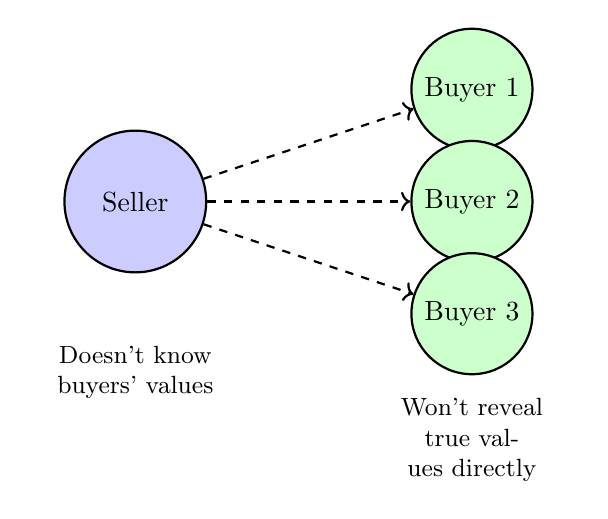
\begin{tikzpicture}[scale=0.95]
  % Seller
  \node[draw, thick, fill=blue!20, circle, minimum size=1.8cm] (seller) at (0,0) {Seller};
  
  % Buyers
  \node[draw, thick, fill=green!20, circle, minimum size=1.3cm] (b1) at (4.5,1.5) {Buyer 1};
  \node[draw, thick, fill=green!20, circle, minimum size=1.3cm] (b2) at (4.5,0) {Buyer 2};
  \node[draw, thick, fill=green!20, circle, minimum size=1.3cm] (b3) at (4.5,-1.5) {Buyer 3};
  
  % Arrows
  \draw[->, thick, dashed] (seller) -- (b1);
  \draw[->, thick, dashed] (seller) -- (b2);
  \draw[->, thick, dashed] (seller) -- (b3);
  
  % Labels
  \node[below, text width=2.5cm, align=center, font=\small] at (0,-1.8) {Doesn't know\\buyers' values};
  \node[below, text width=2.5cm, align=center, font=\small] at (4.5,-2.5) {Won't reveal\\true values directly};
\end{tikzpicture}
\end{center}

\textbf{Solution:} Design an auction that reveals true values through competition
\end{frame}

%===============================================

%===============================================
\part{Foundations}
\partslide
\section{Game-Theoretic Framework}
\sectionslide
%===============================================

\begin{frame}{What Are We Studying? The Auction Game}
\textbf{The Basic Auction Story:}
\begin{itemize}
  \item Multiple people want the same thing
  \item Only one can have it (or limited quantities)
  \item How do we decide who gets it and at what price?
\end{itemize}

\vspace{0.3cm}
\textbf{Why Game Theory?}
\begin{itemize}
  \item Your best strategy depends on what others do
  \item Others' strategies depend on what you do
  \item Everyone is trying to outsmart everyone else
  \item Information is often incomplete or asymmetric
\end{itemize}

\vspace{0.3cm}
\textbf{The Central Questions:}
\begin{itemize}
  \item How should rational bidders behave?
  \item What auction format maximizes seller revenue?
  \item How does information structure affect outcomes?
\end{itemize}
\end{frame}

\begin{frame}{Strategic Form Games}
\textbf{Definition:} A game $\Gamma = \langle N, (S_i)_{i \in N}, (u_i)_{i \in N} \rangle$ consists of:
\begin{itemize}
  \item \textbf{Players:} $N = \{1, 2, \ldots, n\}$
  \item \textbf{Strategy spaces:} $S_i$ for each player $i$
  \item \textbf{Payoff functions:} $u_i: S_1 \times \cdots \times S_n \to \mathbb{R}$
\end{itemize}

\vspace{0.3cm}
\textbf{Solution Concepts:}
\begin{enumerate}
  \item \textbf{Dominant Strategy:} $s_i^* \in S_i$ such that
  \[u_i(s_i^*, s_{-i}) \geq u_i(s_i, s_{-i}) \quad \forall s_i \in S_i, \forall s_{-i}\]
  
  \item \textbf{Nash Equilibrium:} Profile $(s_1^*, \ldots, s_n^*)$ where
  \[u_i(s_i^*, s_{-i}^*) \geq u_i(s_i, s_{-i}^*) \quad \forall s_i \in S_i, \forall i\]
\end{enumerate}
\end{frame}

\begin{frame}{Incomplete Information Games}
\textbf{Harsanyi Transformation:}
\begin{itemize}
  \item Nature determines types $\theta = (\theta_1, \ldots, \theta_n)$
  \item Player $i$ observes only $\theta_i$
  \item Common prior: $\theta \sim F$ where $F$ is common knowledge
  \item Strategy: $s_i: \Theta_i \to S_i$
\end{itemize}

\vspace{0.3cm}
\textbf{Bayesian Nash Equilibrium:}

Strategy profile $(s_1^*, \ldots, s_n^*)$ where each $s_i^*: \Theta_i \to S_i$ satisfies:
\[s_i^*(\theta_i) \in \argmax_{s_i} \mathbb{E}_{\theta_{-i}|\theta_i}[u_i(s_i, s_{-i}^*(\theta_{-i}), \theta)]\]

\vspace{0.3cm}
\textbf{Key Insight:} Each type best responds to beliefs about others' strategies
\end{frame}

\begin{frame}{Mechanism Design: The Inverse Problem}
\textbf{Traditional Economics:}
\begin{itemize}
  \item Given rules/institutions $\rightarrow$ Predict behavior/outcomes
  \item Example: Given auction format $\rightarrow$ Find equilibrium
\end{itemize}

\vspace{0.2cm}
\textbf{Mechanism Design (Hurwicz 1960s):}
\begin{itemize}
  \item Given desired outcome $\rightarrow$ Design rules/institutions
  \item Example: Want revenue maximization $\rightarrow$ Design optimal auction
\end{itemize}

\begin{center}
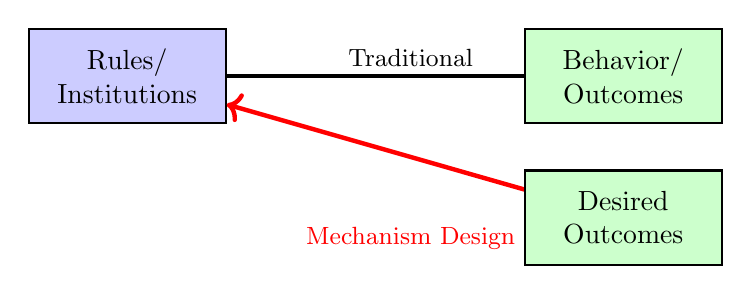
\begin{tikzpicture}[scale=0.9]
  % Traditional box
  \node[draw, thick, fill=blue!20, minimum width=2.5cm, minimum height=1.2cm, align=center] (trad) at (-3,0) {Rules/\\Institutions};
  
  % Arrow
  \draw[->, ultra thick] (trad) -- (4,0);
  \node[above] at (1,0) {\small Traditional};
  
  % Outcomes box
  \node[draw, thick, fill=green!20, minimum width=2.5cm, minimum height=1.2cm, align=center] (out) at (4,0) {Behavior/\\Outcomes};
  
  % Reverse arrow
  \draw[<-, ultra thick, red] (trad) -- (4,-2);
  \node[below] at (1,-2) {\small\color{red} Mechanism Design};
  
  \node[draw, thick, fill=green!20, minimum width=2.5cm, minimum height=1.2cm, align=center] at (4,-2) {Desired\\Outcomes};
\end{tikzpicture}
\end{center}

\textbf{Key Question:} What mechanisms implement desired outcomes?
\end{frame}

\begin{frame}{Direct Mechanisms}
\begin{block}{Definition}
A \textbf{direct mechanism} asks each agent to report their private information (type), then uses these reports to determine:
\begin{itemize}
  \item Allocation: Who gets what
  \item Payments: Who pays what
\end{itemize}
\end{block}

\begin{itemize}
  \item Agent $i$ has type $\theta_i \in \Theta_i$ (e.g., valuation, cost)
  \item Mechanism $(x, p)$: $x: \Theta \to X$ (allocation), $p: \Theta \to \mathbb{R}^n$ (payment)
\end{itemize}

\textbf{Example (Single Item Auction):}
\begin{itemize}
  \item Reports: $\hat{\theta} = (\hat{v}_1, \ldots, \hat{v}_n)$
  \item Allocation: $x_i(\hat{\theta}) = \begin{cases} 1 & \text{if } \hat{v}_i = \max_j \hat{v}_j \\ 0 & \text{otherwise} \end{cases}$
  \item Payment: $p_i(\hat{\theta})$ depends on mechanism
\end{itemize}
\end{frame}

\begin{frame}{Incentive Compatibility and Individual Rationality}
\textbf{Incentive Compatibility (IC):}
\begin{itemize}
  \item Truthful reporting is optimal
  \item Dominant Strategy IC (DSIC): Truth optimal regardless of others
  \vspace{-0.1cm}
  $$U_i(\theta_i, \theta_{-i}) \geq U_i(\hat{\theta}_i, \theta_{-i}) \quad \forall \hat{\theta}_i, \forall \theta_{-i}$$
  \vspace{-0.3cm}
  \item Bayesian IC (BIC): Truth optimal in expectation
  \vspace{-0.1cm}
  $$\E_{\theta_{-i}}[U_i(\theta_i, \theta_{-i})] \geq \E_{\theta_{-i}}[U_i(\hat{\theta}_i, \theta_{-i})] \quad \forall \hat{\theta}_i$$
\end{itemize}
\vspace{-0.2cm}
\textbf{Individual Rationality (IR):}
\begin{itemize}
  \item Voluntary participation
  \item Ex-post IR: $U_i(\theta_i, \theta_{-i}) \geq 0 \quad \forall \theta_{-i}$
  \item Interim IR: $\E_{\theta_{-i}}[U_i(\theta_i, \theta_{-i})] \geq 0$
\end{itemize}
\vspace{-0.1cm}
\textbf{In Auctions:} Second-price: DSIC and ex-post IR; First-price: BIC and interim IR
\end{frame}

\begin{frame}{The Revelation Principle}
\begin{theorem}[Revelation Principle]
For any mechanism and any equilibrium of that mechanism, there exists a direct truthful mechanism that achieves the same allocation and utilities.
\end{theorem}

\begin{proofbox}[Proof Sketch]
\begin{enumerate}
  \item Start with mechanism $M$ and equilibrium strategies $s^*(\theta)$
  \item Construct direct mechanism $M'$: ask for types $\hat{\theta}$, apply $s^*(\hat{\theta})$, run $M$
  \item Truthful reporting optimal: $U_i(\theta_i, M') = U_i(s^*(\theta_i), M)$
\end{enumerate}
\end{proofbox}

\textbf{Implication:} Restrict attention to direct truthful mechanisms!

\textbf{Caveat:} Only works for given equilibrium concept (BNE $\rightarrow$ BIC, Dominant $\rightarrow$ DSIC)
\end{frame}

\begin{frame}{Revelation Principle Illustration}
\begin{center}
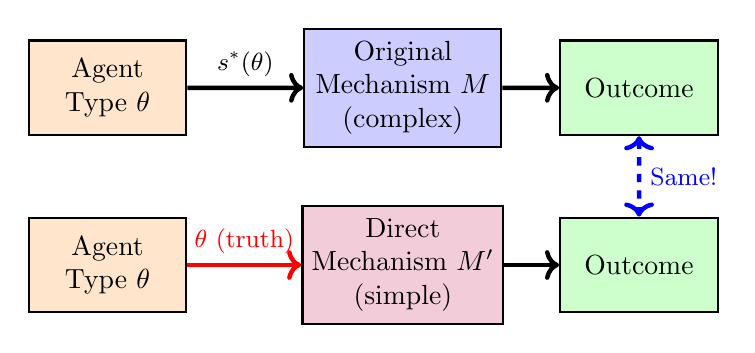
\begin{tikzpicture}[scale=0.75]
  % Original mechanism
  \node[draw, thick, fill=orange!20, minimum width=2cm, minimum height=1.2cm, align=center] (agent1) at (-1,3) {Agent\\Type $\theta$};
  
  \node[draw, thick, fill=blue!20, minimum width=2.5cm, minimum height=1.5cm, align=center] (mech1) at (4,3) {Original\\Mechanism $M$\\(complex)};
  
  \node[draw, thick, fill=green!20, minimum width=2cm, minimum height=1.2cm, align=center] (out1) at (8,3) {Outcome};
  
  \draw[->, ultra thick] (agent1) -- (mech1) node[midway, above, font=\small] {$s^*(\theta)$};
  \draw[->, ultra thick] (mech1) -- (out1);
  
  % Equivalent direct mechanism
  \node[draw, thick, fill=orange!20, minimum width=2cm, minimum height=1.2cm, align=center] (agent2) at (-1,0) {Agent\\Type $\theta$};
  
  \node[draw, thick, fill=purple!20, minimum width=2.5cm, minimum height=1.5cm, align=center] (mech2) at (4,0) {Direct\\Mechanism $M'$\\(simple)};
  
  \node[draw, thick, fill=green!20, minimum width=2cm, minimum height=1.2cm, align=center] (out2) at (8,0) {Outcome};
  
  \draw[->, ultra thick, red] (agent2) -- (mech2) node[midway, above, font=\small, red] {$\theta$ (truth)};
  \draw[->, ultra thick] (mech2) -- (out2);
  
  % Equivalence
  \draw[<->, ultra thick, dashed, blue] (out1) -- (out2) node[midway, right, font=\small] {Same!};
\end{tikzpicture}
\end{center}

\vspace{0.3cm}
\textbf{Designer's Advantage:} Only need to check IC for truthful reporting!
\end{frame}

%===============================================
\section{Order Statistics}
\sectionslide
%===============================================

\begin{frame}{Order Statistics: Essential Theory}
\textbf{Definition:} For i.i.d.\ $X_1, \ldots, X_n \sim F$, order statistics are:
\[X_{(1)} \leq X_{(2)} \leq \cdots \leq X_{(n)}\]

\vspace{0.2cm}
\textbf{Why Important for Auctions?}
\begin{itemize}
  \item Winner has highest valuation: $v_{(n)} = \max\{v_1, \ldots, v_n\}$
  \item Second-price auctions: Winner pays $v_{(n-1)}$
  \item Revenue comparisons require $\mathbb{E}[v_{(n)}]$ and $\mathbb{E}[v_{(n-1)}]$
\end{itemize}

\begin{tcolorbox}[colback=blue!5!white,colframe=blue!75!black,title=Key Result]
For uniform $[0,1]$ distribution:
\[\E[X_{(k)}] = \frac{k}{n+1}, \quad \text{Var}(X_{(k)}) = \frac{k(n-k+1)}{(n+1)^2(n+2)}\]
\end{tcolorbox}
\end{frame}

\begin{frame}{Distribution of Order Statistics}
\textbf{CDF of $k$-th Order Statistic:}
\[G_{(k)}(x) = \sum_{j=k}^n \binom{n}{j} F(x)^j [1-F(x)]^{n-j}\]

\vspace{0.2cm}
\textbf{PDF of $k$-th Order Statistic:}
\[g_{(k)}(x) = \frac{n!}{(k-1)!(n-k)!} F(x)^{k-1}[1-F(x)]^{n-k}f(x)\]

\vspace{0.3cm}
\textbf{Special Cases:}
\begin{itemize}
  \item Maximum: $G_{(n)}(x) = F(x)^n$, \quad $g_{(n)}(x) = nF(x)^{n-1}f(x)$
  \item Minimum: $G_{(1)}(x) = 1-(1-F(x))^n$
  \item Second-highest: $g_{(n-1)}(x) = n(n-1)F(x)^{n-2}[1-F(x)]f(x)$
\end{itemize}
\end{frame}

\begin{frame}{Uniform Distribution: Key Results}
\textbf{For $U[0,1]$ distribution:}

\vspace{0.2cm}
\textbf{General Formula:}
\[\mathbb{E}[X_{(k)}] = \frac{k}{n+1}\]

\vspace{0.3cm}
\textbf{Examples:}
\begin{itemize}
  \item $n=2$: $\mathbb{E}[v_{(2)}] = \frac{2}{3}$, $\mathbb{E}[v_{(1)}] = \frac{1}{3}$
  \item $n=3$: $\mathbb{E}[v_{(3)}] = \frac{3}{4}$, $\mathbb{E}[v_{(2)}] = \frac{1}{2}$
  \item $n=10$: $\mathbb{E}[v_{(10)}] = \frac{10}{11}$, $\mathbb{E}[v_{(9)}] = \frac{9}{11}$
\end{itemize}

\vspace{0.3cm}
\textbf{Intuition:} Order statistics divide $[0,1]$ into $n+1$ equal segments in expectation
\end{frame}

%===============================================
\section{Envelope Theorem}
\sectionslide
%===============================================

\begin{frame}{The Envelope Theorem: Intuition}
\textbf{Standard Optimization:} $V(\theta) = \max_{x} f(x, \theta)$

\textbf{Question:} How does optimal value $V(\theta)$ change with parameter $\theta$?

\textbf{Naive Approach:}
$\frac{dV}{d\theta} = \frac{\partial f}{\partial x}\frac{dx^*}{d\theta} + \frac{\partial f}{\partial \theta}$

\textbf{Envelope Theorem:}
$\frac{dV}{d\theta} = \frac{\partial f}{\partial \theta}\Big|_{x=x^*(\theta)}$

\textbf{Why?} At optimum, $\frac{\partial f}{\partial x} = 0$, so first term vanishes!

\begin{center}
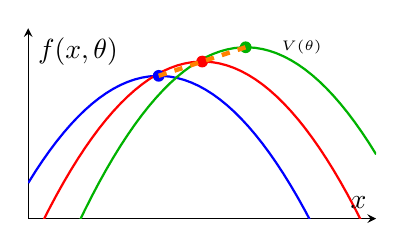
\begin{tikzpicture}[scale=1]
  \begin{axis}[
    xlabel={$x$},
    ylabel={$f(x,\theta)$},
    xmin=0, xmax=4,
    ymin=0, ymax=4,
    axis lines=middle,
    width=6cm,
    height=4cm,
    ticks=none
  ]
  
  % Three parabolas
  \addplot[domain=0:4, samples=50, thick, blue] {-(x-1.5)^2 + 3};
  \addplot[domain=0:4, samples=50, thick, red] {-(x-2)^2 + 3.3};
  \addplot[domain=0:4, samples=50, thick, green!70!black] {-(x-2.5)^2 + 3.6};
  
  % Optimal points
  \node[circle, fill=blue, inner sep=1.5pt] at (axis cs:1.5,3) {};
  \node[circle, fill=red, inner sep=1.5pt] at (axis cs:2,3.3) {};
  \node[circle, fill=green!70!black, inner sep=1.5pt] at (axis cs:2.5,3.6) {};
  
  % Envelope
  \draw[ultra thick, orange, dashed] (axis cs:1.5,3) -- (axis cs:2,3.3) -- (axis cs:2.5,3.6);
  
  \node[right, font=\tiny] at (axis cs:2.8,3.6) {$V(\theta)$};
  
  \end{axis}
\end{tikzpicture}
\end{center}
\end{frame}

%===============================================
\section{Information Structures}
\sectionslide
%===============================================

% \begin{frame}{Type Spaces and Beliefs}
% \textbf{Harsanyi Type Space $(T_i, \tau_i, p_i)_{i \in N}$:}
% \begin{itemize}
%   \item $T_i$: Type space for player $i$
%   \item $\tau_i: \Theta \to T_i$: Type function
%   \item $p_i: T_i \to \Delta(T_{-i} \times \Theta)$: Belief function
% \end{itemize}

% \vspace{0.3cm}
% \textbf{In Auctions:}
% \begin{itemize}
%   \item Type often equals private value: $t_i = v_i$
%   \item Or signal about common value: $t_i = s_i$
%   \item Beliefs derived from common prior $F$
% \end{itemize}
% \end{frame}

\begin{frame}{Types of Information in Auctions}
\textbf{1. Independent Private Values (IPV):}
\begin{itemize}
  \item Each bidder knows own valuation exactly: $v_i$
  \item Values drawn i.i.d.\ from $F$; learning others' values doesn't change own
  \item Example: Personal use items
\end{itemize}

\textbf{2. Common Values (CV):}
\begin{itemize}
  \item Single unknown value $V$ same for all bidders
  \item Each bidder receives private signal $s_i$ about $V$
  \item Winner's curse: Winning means highest estimate
  \item Example: Oil drilling rights
\end{itemize}

\textbf{3. Affiliated Values:}
\begin{itemize}
  \item General case: $v_i = v_i(s_1, \ldots, s_n)$
  \item Signals correlated (higher signal makes high values more likely)
  \item Encompasses both IPV and CV as special cases
\end{itemize}
\end{frame}

\begin{frame}{Value Types Spectrum}
\begin{center}
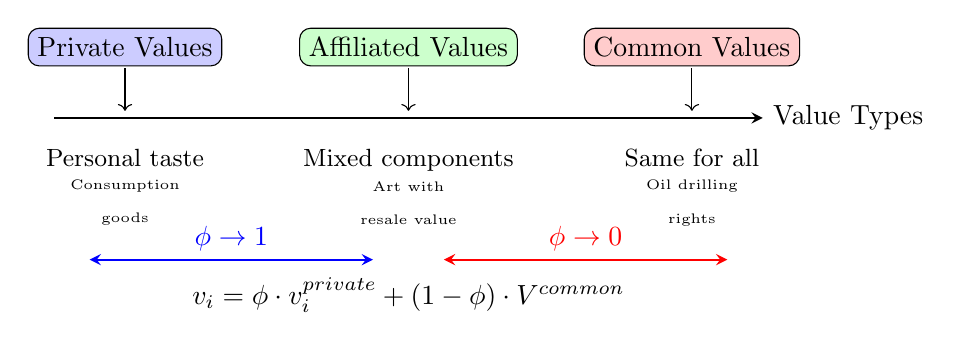
\begin{tikzpicture}[scale=0.9]
  % Spectrum line
  \draw[thick, ->, >=stealth] (0,0) -- (10,0) node[right] {Value Types};
  
  % Private Values
  \node[draw, fill=blue!20, rounded corners] at (1,1) {Private Values};
  \draw[->] (1,0.7) -- (1,0.1);
  \node[below] at (1,-0.3) {\small Personal taste};
  
  % Affiliated Values
  \node[draw, fill=green!20, rounded corners] at (5,1) {Affiliated Values};
  \draw[->] (5,0.7) -- (5,0.1);
  \node[below] at (5,-0.3) {\small Mixed components};
  
  % Common Values
  \node[draw, fill=red!20, rounded corners] at (9,1) {Common Values};
  \draw[->] (9,0.7) -- (9,0.1);
  \node[below] at (9,-0.3) {\small Same for all};
  
  % Examples
  \node[align=center] at (1,-1.2) {\tiny Consumption\\\tiny goods};
  \node[align=center] at (5,-1.2) {\tiny Art with\\\tiny resale value};
  \node[align=center] at (9,-1.2) {\tiny Oil drilling\\\tiny rights};
  
  % Formula
  \node at (5,-2.5) {$v_i = \phi \cdot v_i^{private} + (1-\phi) \cdot V^{common}$};
  \draw[<->, >=stealth, thick, blue] (0.5,-2) -- (4.5,-2);
  \node[blue] at (2.5,-1.7) {$\phi \to 1$};
  \draw[<->, >=stealth, thick, red] (5.5,-2) -- (9.5,-2);
  \node[red] at (7.5,-1.7) {$\phi \to 0$};
\end{tikzpicture}
\end{center}
\end{frame}

%===============================================
\section{Knowledge and Common Knowledge}
\sectionslide
%===============================================

\begin{frame}{Why Knowledge Matters in Auctions}
\textbf{The Information Puzzle:}
\begin{itemize}
  \item In auctions, what you know matters
  \item But what you know that others know also matters
  \item And what you know that others know that you know\ldots
  \item This infinite regress is crucial for strategic reasoning!
\end{itemize}

\vspace{0.3cm}
\textbf{Common Knowledge in Practice:}
\begin{itemize}
  \item Auction rules must be common knowledge
  \item Reserve prices often announced publicly
  \item Some information deliberately kept private
  \item Strategic information revelation can increase revenue
\end{itemize}
\end{frame}

\begin{frame}{Knowledge Operators: Formal Framework}
\textbf{Epistemic Logic:}
\begin{itemize}
  \item Knowledge operator $K_i$: ``agent $i$ knows that\ldots''
  \item $K_i \varphi$ means ``agent $i$ knows proposition $\varphi$''
\end{itemize}

\vspace{0.3cm}
\textbf{S5 Axiom System:}
\begin{enumerate}
  \item \textbf{Truth:} $K_i \varphi \rightarrow \varphi$
  \item \textbf{Positive Introspection:} $K_i \varphi \rightarrow K_i K_i \varphi$
  \item \textbf{Negative Introspection:} $\neg K_i \varphi \rightarrow K_i \neg K_i \varphi$
  \item \textbf{Distribution:} $K_i(\varphi \rightarrow \psi) \rightarrow (K_i \varphi \rightarrow K_i \psi)$
\end{enumerate}

\vspace{0.3cm}
\textbf{Implication:} Agents have perfect knowledge of their own knowledge state
\end{frame}

\begin{frame}{Common Knowledge Definition}
\textbf{Iterative Definition:}
\vspace{-0.2cm}
\begin{align*}
E^1(\varphi) &= \bigwedge_{i \in N} K_i \varphi \quad \text{(everyone knows)} \\
E^k(\varphi) &= E(E^{k-1}(\varphi)) \quad \text{($k$-th level)} \\
C(\varphi) &= \bigwedge_{k=1}^{\infty} E^k(\varphi) \quad \text{(common knowledge)}
\end{align*}
\textbf{In Auctions, Common Knowledge Includes:}
\begin{itemize}
  \item Number of bidders $n$; Auction format and rules
  \item Distribution $F$ (but not realizations); Rationality of all bidders
  \item Reserve price (if public)
\end{itemize}

\textbf{Private Information:}
\begin{itemize}
  \item Own valuation or signal
  \item Own bidding strategy (in sealed-bid)
\end{itemize}
\end{frame}

\begin{frame}{Common Knowledge Illustration}
\begin{figure}[h]
\centering
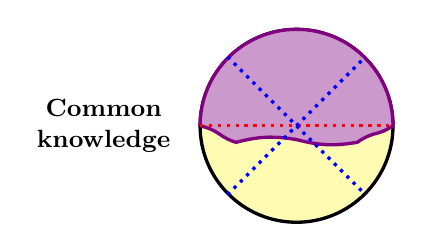
\begin{tikzpicture}[scale=0.35]
    \fill[yellow!30!white] (0,0) circle (3.5cm);
    \draw[very thick, black] (0,0) circle (3.5cm);
    
    % Large purple shape covering the entire top part of the circle
    \draw[very thick, violet, fill=violet!40] 
        (-3.5, 0) arc[start angle=180, end angle=0, radius=3.5cm]
        to[bend left=10] (2.8, -0.3)
        to[bend right=8] (2.2, -0.6)
        to[bend left=12] (0, -0.5)
        to[bend right=12] (-2.2, -0.6)
        to[bend left=8] (-2.8, -0.3)
        to[bend right=10] (-3.5, 0);
    
    % Dotted lines on top
    \draw[red, dotted, very thick] (-3.5, 0) -- (3.5, 0);
    \draw[blue, dotted, very thick] (-2.5, -2.5) -- (2.5, 2.5);
    \draw[blue, dotted, very thick] (-2.5, 2.5) -- (2.5, -2.5);
    
    \node[align=center, font=\small\bfseries] at (-7, 0) {Common\\knowledge};
\end{tikzpicture}
\hspace{0.3cm}
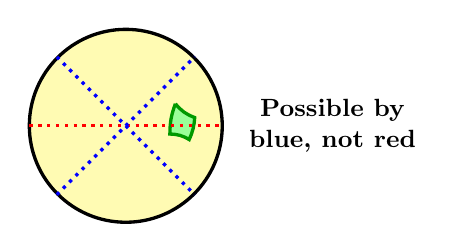
\begin{tikzpicture}[scale=0.35]
    \fill[yellow!30!white] (0,0) circle (3.5cm);
    \draw[very thick, black] (0,0) circle (3.5cm);
    
    % Green shape in the right blue quadrant
    \draw[very thick, green!60!black, fill=green!40] 
        (1.8, 0.8) to[bend right=15] 
        (2.5, 0.3) to[bend left=10] 
        (2.3, -0.5) to[bend right=15] 
        (1.6, -0.3) to[bend left=10] 
        (1.8, 0.8);
    
    \draw[red, dotted, very thick] (-3.5, 0) -- (3.5, 0);
    \draw[blue, dotted, very thick] (-2.5, -2.5) -- (2.5, 2.5);
    \draw[blue, dotted, very thick] (-2.5, 2.5) -- (2.5, -2.5);
    
    \node[align=center, font=\small\bfseries] at (7.5, 0) {Possible by\\blue, not red};
\end{tikzpicture}

\vspace{0.2cm}

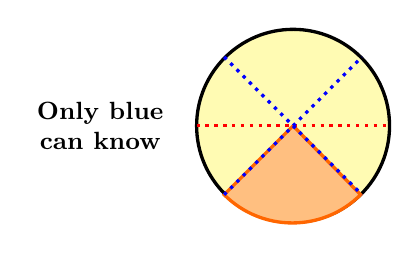
\begin{tikzpicture}[scale=0.35]
    \fill[yellow!30!white] (0,0) circle (3.5cm);
    \draw[very thick, black] (0,0) circle (3.5cm);
    
    % Orange shape in bottom quadrants
    \draw[very thick, orange!80!red, fill=orange!50] 
        (0, 0) -- (-2.5, -2.5) 
        arc[start angle=225, end angle=315, radius=3.5cm] 
        -- cycle;
    
    \draw[red, dotted, very thick] (-3.5, 0) -- (3.5, 0);
    \draw[blue, dotted, very thick] (-2.5, -2.5) -- (2.5, 2.5);
    \draw[blue, dotted, very thick] (-2.5, 2.5) -- (2.5, -2.5);
    
    \node[align=center, font=\small\bfseries] at (-7, 0) {Only blue\\can know};
\end{tikzpicture}
\hspace{0.3cm}
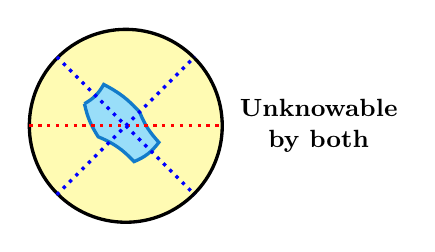
\begin{tikzpicture}[scale=0.35]
    \fill[yellow!30!white] (0,0) circle (3.5cm);
    \draw[very thick, black] (0,0) circle (3.5cm);
    
    % Cyan shape that crosses both partition lines
    \draw[very thick, cyan!60!blue, fill=cyan!40] 
        (-1.5, 0.8) to[bend right=15] 
        (-0.8, 1.5) to[bend left=10] 
        (0.5, 0.5) to[bend right=10] 
        (1.2, -0.6) to[bend left=15] 
        (0.3, -1.3) to[bend right=12] 
        (-1.0, -0.4) to[bend left=10] 
        (-1.5, 0.8);
    
    \draw[red, dotted, very thick] (-3.5, 0) -- (3.5, 0);
    \draw[blue, dotted, very thick] (-2.5, -2.5) -- (2.5, 2.5);
    \draw[blue, dotted, very thick] (-2.5, 2.5) -- (2.5, -2.5);
    
    \node[align=center, font=\small\bfseries] at (7, 0) {Unknowable\\by both};
\end{tikzpicture}
\end{figure}

{\small Blue dotted lines: sharper agent's partition. Red dotted line: coarser agent's partition.}
\end{frame}

\begin{frame}{Mutual Knowledge to Common Knowledge}
\begin{figure}[h]
\centering
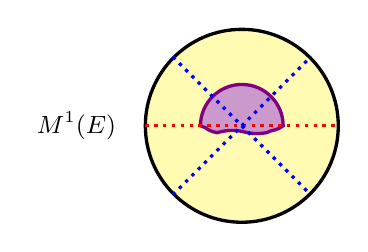
\begin{tikzpicture}[scale=0.35]
    \fill[yellow!30!white] (0,0) circle (3.5cm);
    \draw[very thick, black] (0,0) circle (3.5cm);
    
    \draw[very thick, violet, fill=violet!40] 
        (-1.5, 0) arc[start angle=180, end angle=0, radius=1.5cm]
        to[bend left=10] (1.2, -0.15)
        to[bend right=8] (0.9, -0.25)
        to[bend left=12] (0, -0.2)
        to[bend right=12] (-0.9, -0.25)
        to[bend left=8] (-1.2, -0.15)
        to[bend right=10] (-1.5, 0);
    
    \draw[red, dotted, very thick] (-3.5, 0) -- (3.5, 0);
    \draw[blue, dotted, very thick] (-2.5, -2.5) -- (2.5, 2.5);
    \draw[blue, dotted, very thick] (-2.5, 2.5) -- (2.5, -2.5);
    
    \node[align=center, font=\small\bfseries] at (-6, 0) {$M^1(E)$};
\end{tikzpicture}
\hspace{0.5cm}
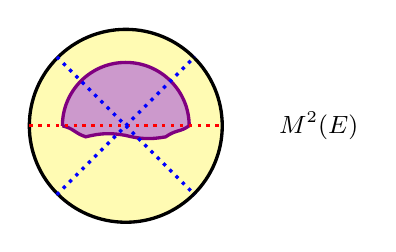
\begin{tikzpicture}[scale=0.35]
    \fill[yellow!30!white] (0,0) circle (3.5cm);
    \draw[very thick, black] (0,0) circle (3.5cm);
    
    \draw[very thick, violet, fill=violet!40] 
        (-2.3, 0) arc[start angle=180, end angle=0, radius=2.3cm]
        to[bend left=10] (1.85, -0.2)
        to[bend right=8] (1.45, -0.4)
        to[bend left=12] (0, -0.35)
        to[bend right=12] (-1.45, -0.4)
        to[bend left=8] (-1.85, -0.2)
        to[bend right=10] (-2.3, 0);
    
    \draw[red, dotted, very thick] (-3.5, 0) -- (3.5, 0);
    \draw[blue, dotted, very thick] (-2.5, -2.5) -- (2.5, 2.5);
    \draw[blue, dotted, very thick] (-2.5, 2.5) -- (2.5, -2.5);
    
    \node[align=center, font=\small\bfseries] at (7, 0) {$M^2(E)$};
\end{tikzpicture}

\vspace{0.3cm}

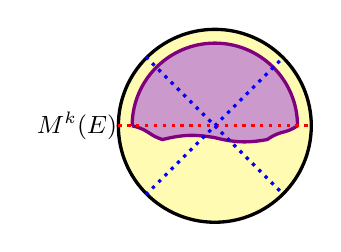
\begin{tikzpicture}[scale=0.35]
    \fill[yellow!30!white] (0,0) circle (3.5cm);
    \draw[very thick, black] (0,0) circle (3.5cm);
    
    \draw[very thick, violet, fill=violet!40] 
        (-3.0, 0) arc[start angle=180, end angle=0, radius=3.0cm]
        to[bend left=10] (2.4, -0.25)
        to[bend right=8] (1.9, -0.5)
        to[bend left=12] (0, -0.43)
        to[bend right=12] (-1.9, -0.5)
        to[bend left=8] (-2.4, -0.25)
        to[bend right=10] (-3.0, 0);
    
    \draw[red, dotted, very thick] (-3.5, 0) -- (3.5, 0);
    \draw[blue, dotted, very thick] (-2.5, -2.5) -- (2.5, 2.5);
    \draw[blue, dotted, very thick] (-2.5, 2.5) -- (2.5, -2.5);
    
    \node[align=center, font=\small\bfseries] at (-5, 0) {$M^k(E)$};
\end{tikzpicture}
\hspace{0.5cm}
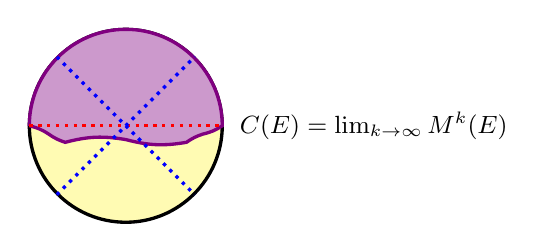
\begin{tikzpicture}[scale=0.35]
    \fill[yellow!30!white] (0,0) circle (3.5cm);
    \draw[very thick, black] (0,0) circle (3.5cm);
    
    \draw[very thick, violet, fill=violet!40] 
        (-3.5, 0) arc[start angle=180, end angle=0, radius=3.5cm]
        to[bend left=10] (2.8, -0.3)
        to[bend right=8] (2.2, -0.6)
        to[bend left=12] (0, -0.5)
        to[bend right=12] (-2.2, -0.6)
        to[bend left=8] (-2.8, -0.3)
        to[bend right=10] (-3.5, 0);
    
    \draw[red, dotted, very thick] (-3.5, 0) -- (3.5, 0);
    \draw[blue, dotted, very thick] (-2.5, -2.5) -- (2.5, 2.5);
    \draw[blue, dotted, very thick] (-2.5, 2.5) -- (2.5, -2.5);
    
    \node[align=center, font=\small\bfseries] at (9, 0) {$C(E) = \lim_{k \to \infty} M^k(E)$};
\end{tikzpicture}
\end{figure}

\vspace{0.2cm}
{\small $M^k(E)$: ``Everyone knows that everyone knows that\ldots ($k$ times)\ldots that $E$ occurred.''}
\end{frame}

%===============================================
\part{Single Item}
\partslide
%===============================================
\section{Key Assumptions}
%===============================================

\begin{frame}{Benchmark Model Setup}
\textbf{Three Key Assumptions:}
\begin{enumerate}
  \item \textbf{Independent Private Values (IPV):} 
  \begin{itemize}
    \item Valuations statistically independent
    \item Learning others' values doesn't change own value
  \end{itemize}
  \item \textbf{Risk Neutrality:} 
  \begin{itemize}
    \item Utility $U_i = v_i - p_i$ if win, 0 if lose
    \item No risk aversion or risk seeking
  \end{itemize}
  \item \textbf{Symmetry:} 
  \begin{itemize}
    \item All bidders from same distribution $F$
    \item No ex-ante differences between bidders
  \end{itemize}
\end{enumerate}

\textbf{Notation:}
\begin{itemize}
  \item $n$ bidders, valuations $v_i \sim F(v)$ on $[\underline{v}, \bar{v}]$
  \item Density $f(v) = F'(v)$, assume $f > 0$ on support
  \item Order statistics: $v_{(1)} \geq v_{(2)} \geq \cdots \geq v_{(n)}$
  \item Seller's valuation: $v_s = 0$ (for simplicity)
\end{itemize}
\end{frame}

\begin{frame}{Overview: Six Standard Formats}
Let $v$ = your valuation, $b$ = your bid, $b_1$ = highest bid, $b_2$ = 2nd-highest

\begin{enumerate}
  \item \textbf{English (Ascending Price)}
  \item \textbf{Dutch (Descending Price)}
  \item \textbf{Sealed-Bid First-Price:} $\pi = \mathbb{P}(b = b_1) \cdot (v - b)$
  \item \textbf{Sealed-Bid Second-Price:} $\pi = \mathbb{P}(b = b_1) \cdot (v - b_2)$
  \item \textbf{All-Pay First Price:} $\pi = \mathbb{P}(b = b_1) \cdot v - b$
  \item \textbf{All-Pay Second Price:} $\pi = \mathbb{P}(b = b_1) \cdot (v - b_2) - \mathbb{P}(b \neq b_1) \cdot b$
\end{enumerate}

\textbf{We'll cover:} Definition, equilibrium, derivation for each format
\end{frame}

\section{English Auction}

\begin{frame}{English Auction: Definition}
\begin{block}{Definition}
An \textbf{English auction} is a sequential mechanism where bidders indicate interest at a current price. Price increases incrementally until only one bidder remains.
\end{block}

\textbf{Standard Ascending Format:}
\begin{itemize}
\item Prices increase incrementally
\item Bidders signal their interest
\item Ends when only one bidder signals
\item Only winner pays (pays final price)
\end{itemize}

\textbf{Reverse English (Procurement):}
\begin{itemize}
\item Prices decrease incrementally
\item Bidders signal willingness to sell
\item Ends when only one bidder signals
\end{itemize}
\end{frame}

\begin{frame}{English Auction: Equilibrium}
\textbf{Dominant Strategy:}
\begin{itemize}
  \item Stay in auction while price $p < v_i$
  \item Drop out when price $p \geq v_i$
  \item Strategy independent of beliefs about others
\end{itemize}

\textbf{Equilibrium Outcome:}
\begin{itemize}
  \item Bidder with $v_{(2)}$ drops out at $p = v_{(2)}$
  \item Bidder with $v_{(1)}$ wins
  \item Pays price $p = v_{(2)}$
  \item Winner's surplus: $v_{(1)} - v_{(2)} > 0$
\end{itemize}

\textbf{Properties:}
\begin{itemize}
  \item \textcolor{green}{Efficient (highest value wins)}
  \item Simple strategy (no need to know $F$ or $n$)
  \item Transparent process
  \item Information revelation as bidders drop out
\end{itemize}
\end{frame}

\begin{frame}{English Auction: Proof of Dominance}
\textbf{Claim:} Staying active while $p < v_i$ is weakly dominant

\textbf{Proof:} Consider bidder $i$ with value $v_i$, current price $p$

\textbf{Case 1:} $p < v_i$
\begin{itemize}
  \item Stay active: Win if others drop first, payoff $= v_i - p_{final} \geq v_i - p > 0$
  \item Drop out: Lose, payoff $= 0$
  \item Staying dominates dropping
\end{itemize}

\textbf{Case 2:} $p \geq v_i$
\begin{itemize}
  \item Stay active: If win, pay $p \geq v_i$, payoff $\leq 0$
  \item Drop out: Lose, payoff $= 0$
  \item Dropping (weakly) dominates staying
\end{itemize}

\textbf{Equilibrium Bidding:} $b(v_i) = v_i$ (stay until price reaches value)

\textbf{Winner pays:} $p^* = v_{(2)}$
\end{frame}

\section{Second-Price Sealed-Bid}

\begin{frame}{Second-Price Auction: Definition}
\begin{block}{Definition}
A \textbf{second-price (Vickrey) auction} is a simultaneous mechanism where the highest bidder wins but pays the second-highest bid.
\end{block}

\textbf{Sealed-Bid Second-Price Format:}
\begin{itemize}
\item Bidders submit sealed bids simultaneously
\item Highest bid wins the item
\item Winner pays the second-highest bid
\item Only winner pays
\end{itemize}

\begin{alertblock}{Strategic Property}
Bidding your true valuation is a dominant strategy—no incentive to bid higher or lower.
\end{alertblock}
\end{frame}

\begin{frame}{Second-Price: Dominant Strategy Theorem}
\begin{theorem}[Dominant Strategy]
In a second-price sealed-bid auction, bidding true valuation $b_i = v_i$ is a weakly dominant strategy for all bidders.
\end{theorem}

\textbf{Proof:} Let $\tilde{b} = \max_{j \neq i} b_j$ (highest other bid)

\textbf{Case 1: Overbidding} $(b > v)$
\begin{itemize}
    \item If $\tilde{b}> v$: Don't want to win (would pay $> v$)
    \item If $\tilde{b}< v$: Win by bidding $b=v$ too, same payoff $v-\tilde{b}>0$
    \item Bidding $v$ dominates: avoids losses, keeps gains
\end{itemize}

\textbf{Case 2: Underbidding} $(b < v)$
\begin{itemize}
  \item If $v > \tilde{b} > b$: Lose, but could win profitably
  \item If $v > b > \tilde{b}$: Win with same profit as bidding $v$ 
  \item Bidding $v$ dominates: captures all opportunities
\end{itemize}

$\square$
\end{frame}

\section{First-Price Sealed-Bid}

\begin{frame}{First-Price Auction: Definition}
\begin{block}{Definition}
A \textbf{first-price auction} is a simultaneous mechanism where the highest bidder wins and pays their own bid.
\end{block}

\textbf{Sealed-Bid First-Price Format:}
\begin{itemize}
\item Bidders submit sealed bids
\item Highest bid wins the item
\item Winner pays their own bid
\item Only winner pays
\end{itemize}

\begin{alertblock}{Strategic Challenge}
Bidders face a trade-off: bidding high increases win probability but decreases profit if winning. This is the \textbf{bid-shading problem}.
\end{alertblock}
\end{frame}

\begin{frame}{First-Price: The Trade-off}
\begin{center}
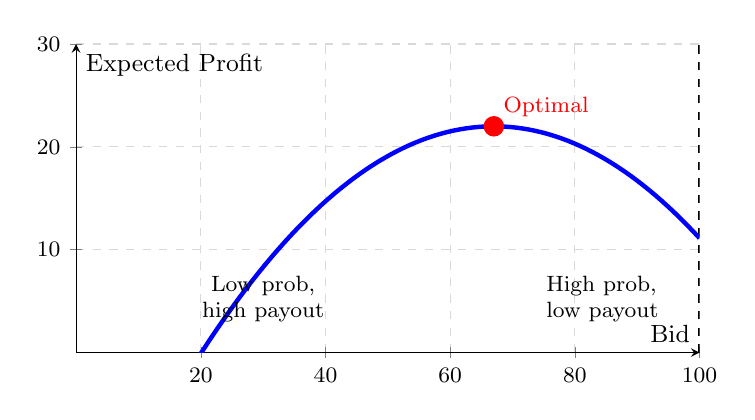
\begin{tikzpicture}[scale=1]
  \begin{axis}[
    xlabel={Bid},
    ylabel={Expected Profit},
    xmin=0, xmax=100,
    ymin=0, ymax=30,
    axis lines=middle,
    width=9.5cm,
    height=5.5cm,
    grid=major,
    grid style={dashed, gray!30},
    xtick={0,20,40,60,80,100},
    ytick={0,10,20,30},
    xlabel style={font=\small},
    ylabel style={font=\small},
    tick label style={font=\footnotesize}
  ]
  
  % True value line
  \addplot[domain=0:100, samples=2, very thick, black, dashed] coordinates {(100,0) (100,30)};
  \node[font=\footnotesize] at (axis cs:100,32) {Your Value \$100K};
  
  % Expected profit curve
  \addplot[domain=0:100, samples=100, ultra thick, blue] {-0.01*(x-67)^2 + 22};
  
  % Optimal bid marker
  \addplot[mark=*, mark size=3.5pt, only marks, red] coordinates {(67,22)};
  \node[above right, red, font=\footnotesize] at (axis cs:67,22) {Optimal};
  
  % Annotations
  \node[above, align=center, font=\footnotesize] at (axis cs:30,2) {Low prob,\\high payout};
  \node[above left, align=left, font=\footnotesize] at (axis cs:95,2) {High prob,\\low payout};
  
  \end{axis}
\end{tikzpicture}
\end{center}

\textbf{Key Insight:} Higher bid increases win chance but reduces profit
\end{frame}

\begin{frame}{First-Price: Equilibrium Derivation}
\textbf{Setup:} If bidder $i$ with value $v_i$ bids as if value $w_i$:
$$\E[U_i] = (v_i - B(w_i)) \cdot F^{n-1}(w_i)$$

\textbf{First-Order Condition:}
$$\frac{\partial}{\partial w_i}: (v_i - B(w_i))(n-1)f(w_i)F^{n-2}(w_i) - B'(w_i)F^{n-1}(w_i) = 0$$

At symmetric equilibrium $w_i = v_i$:
$$B'(v_i) = (n-1)(v_i - B(v_i))\frac{f(v_i)}{F(v_i)}$$

\textbf{General Solution} (with $B(\underline{v}) = \underline{v}$):
$$B(v_i) = \frac{\int_{\underline{v}}^{v_i} t \, dF^{n-1}(t)}{F^{n-1}(v_i)} = v_i - \frac{\int_{\underline{v}}^{v_i} F^{n-1}(t)dt}{F^{n-1}(v_i)}$$

\textbf{Note:} $B(v_i) < v_i$ (always shade bid below value)
\end{frame}

\begin{frame}{First-Price: Uniform Example}
\textbf{Setup:} $v \sim U[0,1]$, so $F(v) = v$, $f(v) = 1$

\textbf{Differential equation:}
$$B'(v_i) = \frac{(n-1)(v_i - B(v_i))}{v_i}$$

\textbf{Guess linear solution:} $B(v_i) = kv_i$

Substituting: $k = \frac{(n-1)(v_i - kv_i)}{v_i} = (n-1)(1-k)$

Solving: $k = \frac{n-1}{n}$

\textbf{Equilibrium bid function:}
$$\boxed{B(v_i) = \frac{n-1}{n} v_i}$$

\textbf{Examples:}
\begin{itemize}
  \item 2 bidders: bid 50\% of value
  \item 10 bidders: bid 90\% of value  
  \item As $n \to \infty$: $B(v) \to v$ (competition eliminates shading)
\end{itemize}
\end{frame}

\section{Dutch Auction}

\begin{frame}{Dutch Auction: Definition}
\begin{block}{Definition}
A \textbf{Dutch auction} is a sequential mechanism where an auctioneer decreases the price until the first bidder signals acceptance.
\end{block}

\textbf{Standard Descending Format:}
\begin{itemize}
\item Prices decrease incrementally
\item Bidders watch and wait
\item First to accept wins at current price
\item Only winner pays
\end{itemize}

\textbf{Reverse Dutch (Procurement):}
\begin{itemize}
\item Prices increase incrementally
\item First seller to accept wins
\end{itemize}
\end{frame}

\begin{frame}{Claim: Dutch and First-Price auctions are strategically equivalent}
\textbf{Dutch Decision:}
\begin{itemize}
  \item Choose stopping price $b$ before auction starts
  \item Accept when clock reaches $b$
  \item If someone else accepts first, lose
  \item Payoff: $(v_i - b) \cdot \mathbb{P}(b > \max_{j \neq i} b_j)$
\end{itemize}

\textbf{First-Price Decision:}
\begin{itemize}
  \item Choose bid $b$ to submit in sealed envelope
  \item If $b$ is highest, win and pay $b$
  \item Otherwise lose
  \item Payoff: $(v_i - b) \cdot \mathbb{P}(b > \max_{j \neq i} b_j)$
\end{itemize}

\textbf{Why Equivalent? Same:}
\begin{itemize}
  \item Information at decision time (only own value); Action space (choose a price)
  \item Payoff structures
  \item $\Rightarrow$ Identical equilibrium strategies: $b_{Dutch}(v_i) = b_{First}(v_i)$
\end{itemize}
\end{frame}


\section{All-Pay Auctions}
%===============================================

\begin{frame}{All-Pay First-Price: Definition}
\begin{block}{Definition}
An \textbf{all-pay first-price auction} is a simultaneous mechanism where the highest bidder wins, but \textbf{all bidders pay their bids}.
\end{block}

\textbf{Format:}
\begin{itemize}
\item Bidders submit sealed bids
\item Highest bid wins the item
\item \textbf{All bidders pay their bids} (winners and losers)
\item Winner receives item, losers receive nothing
\end{itemize}

\textbf{Applications:}
\begin{itemize}
  \item R\&D races (all firms invest, one wins patent)
  \item Political lobbying (all parties spend, one wins favor)
  \item Legal contests (all parties pay fees, one wins case)
\end{itemize}
\end{frame}

\begin{frame}{All-Pay First-Price: The Challenge}
\begin{center}
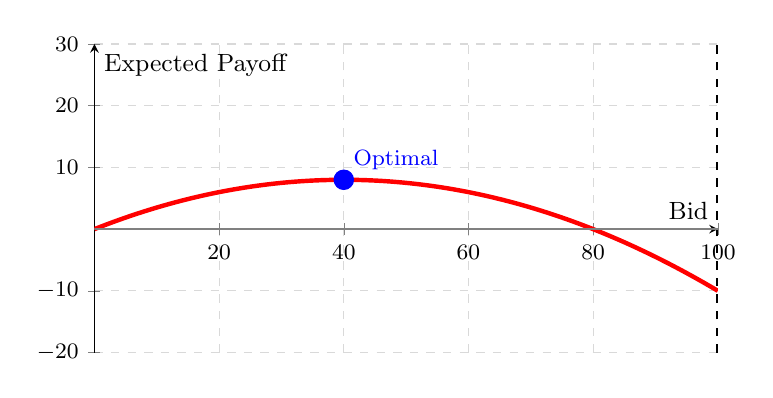
\begin{tikzpicture}[scale=1]
  \begin{axis}[
    xlabel={Bid},
    ylabel={Expected Payoff},
    xmin=0, xmax=100,
    ymin=-20, ymax=30,
    axis lines=middle,
    width=9.5cm,
    height=5.5cm,
    grid=major,
    grid style={dashed, gray!30},
    xtick={0,20,40,60,80,100},
    ytick={-20,-10,0,10,20,30},
    xlabel style={font=\small},
    ylabel style={font=\small},
    tick label style={font=\footnotesize}
  ]
  
  % Value line
  \addplot[domain=0:100, samples=2, very thick, black, dashed] coordinates {(100,-20) (100,30)};
  \node[font=\footnotesize] at (axis cs:100,32) {Value \$100K};
  
  % Expected payoff curve
  \addplot[domain=0:100, samples=100, ultra thick, red] {-0.005*(x-40)^2 + 8};
  
  % Optimal bid
  \addplot[mark=*, mark size=3.5pt, only marks, blue] coordinates {(40,8)};
  \node[above right, blue, font=\footnotesize] at (axis cs:40,8) {Optimal};
  
  % Zero line
  \addplot[domain=0:100, samples=2, thick, gray] coordinates {(0,0) (100,0)};
  
  \end{axis}
\end{tikzpicture}
\end{center}

\textbf{Key Insight:} Since you pay even if you lose, optimal bids are much lower than standard auctions
\end{frame}

\begin{frame}{All-Pay First-Price: Equilibrium}
\textbf{Symmetric Equilibrium:}
$$b(v_i) = \int_{\underline{v}}^{v_i} t dF^{n-1}(t) = v_i F^{n-1}(v_i) - \int_{\underline{v}}^{v_i} F^{n-1}(t)dt$$

\textbf{Uniform $[0,1]$ Case:}
$$\boxed{b(v_i) = \frac{n-1}{n} v_i^n}$$

\textbf{Comparison to First-Price:}
\begin{itemize}
  \item First-price: $b_{FPA}(v_i) = \frac{n-1}{n} v_i$
  \item All-pay: $b_{AP}(v_i) = \frac{n-1}{n} v_i^n$
  \item Note: $b_{AP}(v_i) < b_{FPA}(v_i)$ for all $v_i < 1$
\end{itemize}

\textbf{Revenue Equivalence Still Holds:}
$$ER_{All-Pay} = \E[v_{(2)}]$$
(All pay, but pay less per person)
hy Revenue Equals \end{frame}

\begin{frame}{All-Pay First-Price: Derivation}
\textbf{Expected Utility:} If bidder with value $v_i$ bids as if value $w$:
\begin{align*}
U(w; v_i) &= v_i \cdot F^{n-1}(w) - B(w) \\
\frac{\partial U}{\partial w} &= v_i(n-1)f(w)F^{n-2}(w) - B'(w) = 0
\end{align*}

At symmetric equilibrium $(w = v_i)$:
$$B'(v_i) = v_i(n-1)f(v_i)F^{n-2}(v_i)$$

Integrating with $B(\underline{v}) = 0$:
$$B(v_i) = \int_{\underline{v}}^{v_i} t \, dF^{n-1}(t) = v_i F^{n-1}(v_i) - \int_{\underline{v}}^{v_i} F^{n-1}(t) \, dt$$

\textbf{Uniform Distribution:}
$$B(v_i) = v_i^n - \frac{v_i^n}{n} = \frac{n-1}{n} v_i^n$$
\end{frame}


\begin{frame}{Information Flow in Different Formats}
\begin{center}
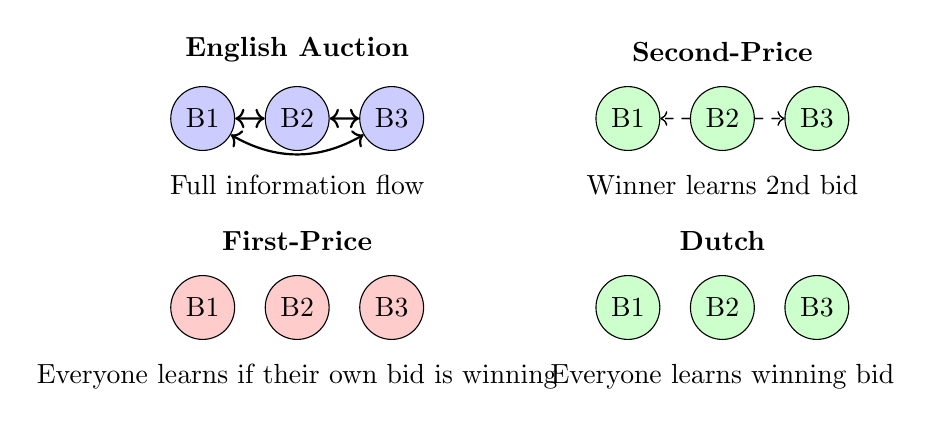
\begin{tikzpicture}[scale=0.6]
  % English Auction
  \node[draw, circle, fill=blue!20] (e1) at (-2,4) {B1};
  \node[draw, circle, fill=blue!20] (e2) at (0,4) {B2};
  \node[draw, circle, fill=blue!20] (e3) at (2,4) {B3};
  \node[above] at (0,5) {\textbf{English Auction}};
  \draw[<->, thick] (e1) -- (e2);
  \draw[<->, thick] (e2) -- (e3);
  \draw[<->, thick] (e1) to[bend right] (e3);
  \node[below] at (0,3) {Full information flow};
  
  % Second-Price
  \node[draw, circle, fill=green!20] (s1) at (7,4) {B1};
  \node[draw, circle, fill=green!20] (s2) at (9,4) {B2};
  \node[draw, circle, fill=green!20] (s3) at (11,4) {B3};
  \node[above] at (9,5) {\textbf{Second-Price}};
  \draw[->, dashed] (s2) -- (s1);
  \draw[->, dashed] (s2) -- (s3);
  \node[below] at (9,3) {Winner learns 2nd bid};
  
  % First-Price
  \node[draw, circle, fill=red!20] (f1) at (-2,0) {B1};
  \node[draw, circle, fill=red!20] (f2) at (0,0) {B2};
  \node[draw, circle, fill=red!20] (f3) at (2,0) {B3};
  \node[above] at (0,1) {\textbf{First-Price}};
  \node[below] at (0,-1) {Everyone learns if their own bid is winning};

  % Dutch auction
  \node[draw, circle, fill=green!20] (d1) at (7,0) {B1};
  \node[draw, circle, fill=green!20] (d2) at (9,0) {B2};
  \node[draw, circle, fill=green!20] (d3) at (11,0) {B3};
  \node[above] at (9,1) {\textbf{Dutch}};
  \draw[->, dashed] (s2) -- (s1);
  \draw[->, dashed] (s2) -- (s3);
  \node[below] at (9,-1) {Everyone learns winning bid};
\end{tikzpicture}
\end{center}
\textbf{Information Revelation Impact:}
\begin{itemize}
  \item More information $\rightarrow$ Less winner's curse
  \item Less winner's curse $\rightarrow$ More aggressive bidding
  \item More aggressive bidding $\rightarrow$ Higher revenue
\end{itemize}
\end{frame}

\section{War of Attrition}

\begin{frame}{War of Attrition: Definition}
\begin{block}{Definition}
A \textbf{war of attrition} (all-pay second-price) is a simultaneous mechanism where the highest bidder wins and pays the second-highest bid, but all losing bidders also pay their own bids.
\end{block}

\textbf{Format:}
\begin{itemize}
\item Bidders submit sealed bids
\item Highest bid wins the item
\item Winner pays the \textbf{second-highest bid}
\item \textbf{All losers pay their own bids}
\end{itemize}

\textbf{Applications:}
\begin{itemize}
  \item Standards wars (all invest, winner sets standard)
  \item Animal contests (all expend energy, winner gets resource)
  \item Market entry battles
\end{itemize}
\end{frame}

\begin{frame}{War of Attrition: Equilibrium}
\textbf{Equilibrium Strategy:}
$$b(v_i) = -v_i \ln(1 - F^{n-1}(v_i)) + \int_{\underline{v}}^{v_i} \ln(1 - F^{n-1}(t))dt$$

\textbf{Two-Player Uniform $[0,1]$ Case:}
$$\boxed{b(v_i) = -v_i + - \ln(1-v_i)}$$

\textbf{Key Properties:}
\begin{itemize}
  \item $\lim_{v_i \to 1} b(v_i) = 1$ (highest type bids their value)
  \item More aggressive than all-pay first-price
  \item Revenue equivalence: $ER_{War} = \E[v_{(2)}]$
\end{itemize}
\end{frame}

\begin{frame}{War of Attrition: Derivation (1)}
\textbf{Expected Utility:}
$$U(w; v_i) = F^{n-1}(w) \cdot v_i - \int_{\underline{v}}^w B(t) dF^{n-1}(t) - (1-F^{n-1}(w))B(w)$$

\textbf{First-Order Condition:}
\begin{align*}
\frac{\partial U}{\partial w} &= (n-1)f(w)F^{n-2}(w)v_i - B(w)(n-1)f(w)F^{n-2}(w) \\
&\quad + (n-1)f(w)F^{n-2}(w)B(w) - B'(w)(1-F^{n-1}(w)) = 0
\end{align*}

At $w = v_i$:
$$B'(v_i)(1-F^{n-1}(v_i)) = (n-1)f(v_i)F^{n-2}(v_i)v_i$$

$$B'(v_i) = \frac{(n-1)f(v_i)F^{n-2}(v_i)}{1-F^{n-1}(v_i)} v_i$$
\end{frame}

\begin{frame}{War of Attrition: Derivation (2)}
Note that:
$$\frac{d}{dv}[-\ln(1-F^{n-1}(v))] = \frac{(n-1)f(v)F^{n-2}(v)}{1-F^{n-1}(v)}$$

Therefore:
$$B'(v_i) = -v_i \frac{d}{dv_i}\ln(1-F^{n-1}(v_i))$$

Integrating by parts with $B(\underline{v}) = 0$:
$$B(v_i) = -v_i\ln(1-F^{n-1}(v_i)) + \int_{\underline{v}}^{v_i} \ln(1-F^{n-1}(t)) \, dt$$

\textbf{Two-Player Uniform Case:}
$$B(v_i) = -v_i\ln(1-v_i) + \int_0^{v_i} \ln(1-t) \, dt = v_i + (1-v_i)\ln(1-v_i)$$
\end{frame}

\section{Contests}
\sectionslide

\begin{frame}{Tullock Contests}
\textbf{Contest Success Function:}
$$p_i(x_i, x_{-i}) = \begin{cases}
\frac{x_i^r}{\sum_{j=1}^n x_j^r} & \text{if } \sum_j x_j > 0 \\
\frac{1}{n} & \text{otherwise}
\end{cases}$$

\textbf{Parameter $r$ (decisiveness):}
\begin{itemize}
\item $r \to 0$: Random lottery (effort irrelevant)
\item $r = 1$: Linear contest
\item $r \to \infty$: All-pay auction (deterministic)
\end{itemize}

\textbf{Symmetric Equilibrium:}
$$\boxed{x^* = \frac{r(n-1)V}{n^2}}$$

\textbf{Rent Dissipation:}
Total effort = $\frac{r(n-1)}{n} \times V$ (fraction of prize value)

\textbf{Existence:} Requires $r \leq 2$ for $n \geq 2$
\end{frame}

\begin{frame}{Tullock: Derivation}
\begin{align*}
\textbf{Expected Utility:}&\quad &&U_i= \frac{x_i^r}{x_i^r + \sum_{j \neq i} x_j^r} \cdot V - x_i \\
\text{In symmetric equilibrium ($x_j = x^*$ for all $j \neq i$):}&\quad &&U_i= \frac{x_i^r}{x_i^r + (n-1)(x^*)^r} \cdot V - x_i \\
\textbf{FOC:}&\quad &&1= \frac{r x_i^{r-1} \cdot (n-1)(x^*)^r}{[x_i^r + (n-1)(x^*)^r]^2} \cdot V \\
\text{At $x_i = x^*$:}&\quad &&1= \frac{V \cdot r(n-1)(x^*)^{2r-1}}{[n \cdot x^*]^{2r}}  \\
\text{Solving:}&\quad &&x^*= \frac{r(n-1)V}{n^2}
\end{align*}
\end{frame}

\begin{frame}{Rank-Order Tournaments}
\textbf{Lazear-Rosen (1981) Model:}
\begin{itemize}
  \item Two workers, output: $q_i = e_i + \varepsilon_i + \theta$
  \item $\varepsilon_i$: Idiosyncratic shock
  \item $\theta$: Common shock
  \item Prizes: $w_1 > w_2$ (winner and loser)
\end{itemize}

\textbf{Tournament Rule:} Worker $i$ wins if $q_i > q_j$

\textbf{Equilibrium Effort:}
$$e^* = \frac{u(w_1) - u(w_2)}{\sigma_\varepsilon \cdot 2\sqrt{\pi}}$$

\textbf{Key Result:}
\begin{itemize}
  \item Tournament dominates piece-rate when common shock large
  \item Piece-rate dominates when idiosyncratic shock large
  \item Tournament filters common shocks via relative performance
\end{itemize}
\end{frame}

\begin{frame}{Proof of Tournament Equilibrium (1/2)}
\textbf{Worker $i$'s Optimization Problem:}

Given $q_i = e_i + \varepsilon_i + \theta$ and $q_j = e_j + \varepsilon_j + \theta$, worker $i$ wins if:
$$q_i > q_j \quad \Leftrightarrow \quad e_i - e_j > \varepsilon_j - \varepsilon_i$$

\textbf{Assumptions:}
\begin{itemize}
  \item $\varepsilon_i \sim N(0, \sigma_\varepsilon^2)$ i.i.d.
  \item Cost of effort: $c(e_i) = e_i$ (linear cost)
  \item Common shock $\theta$ cancels in relative comparison
\end{itemize}

\textbf{Probability of Winning:}
$$\varepsilon_j - \varepsilon_i \sim N(0, 2\sigma_\varepsilon^2)$$
$$P(\text{worker } i \text{ wins}) = \Phi\left(\frac{e_i - e_j}{\sqrt{2}\sigma_\varepsilon}\right)$$

where $\Phi(\cdot)$ is the standard normal CDF.
\end{frame}

\begin{frame}{Proof of Tournament Equilibrium (2/2)}
\small
\begin{align*}
&\max_{e_i}~ \Phi\left(\frac{e_i - e_j}{\sqrt{2}\sigma_\varepsilon}\right) u(w_1) + \left[1 - \Phi\left(\frac{e_i - e_j}{\sqrt{2}\sigma_\varepsilon}\right)\right] u(w_2) - e_i \\[0.8ex]
&\textbf{First-Order Condition:}~ \phi\left(\frac{e_i - e_j}{\sqrt{2}\sigma_\varepsilon}\right) \cdot \frac{1}{\sqrt{2}\sigma_\varepsilon} [u(w_1) - u(w_2)] = 1 \\[0.8ex]
&\text{where } \phi(x) = \frac{1}{\sqrt{2\pi}}e^{-x^2/2} \text{ is the standard normal PDF.} \\[0.8ex]
&\textbf{Symmetric Eq.:}~ e_i = e_j = e^* \implies \phi(0) \cdot \frac{1}{\sqrt{2}\sigma_\varepsilon} [u(w_1) - u(w_2)] = 1 \\[0.8ex]
&\hspace{2.5cm} \frac{1}{\sqrt{2\pi}} \cdot \frac{1}{\sqrt{2}\sigma_\varepsilon} [u(w_1) - u(w_2)] = 1 \\[0.8ex]
&\hspace{2.5cm} \boxed{e^* = \frac{u(w_1) - u(w_2)}{\sigma_\varepsilon \cdot 2\sqrt{\pi}}}
\end{align*}
\end{frame}


\begin{frame}{Visualization: Bid Functions Across Auction Types}
\begin{center}
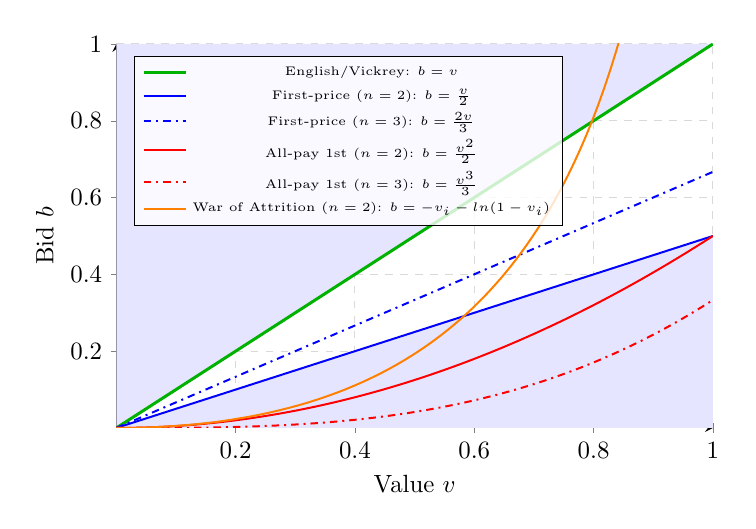
\begin{tikzpicture}[scale=0.9]
  \begin{axis}[
    xlabel={Value $v$},
    ylabel={Bid $b$},
    xmin=0, xmax=1,
    ymin=0, ymax=1,
    axis lines=middle,
    legend pos=north west,
    legend style={font=\tiny, fill=white, fill opacity=0.8, text opacity=1},
    width=10cm,
    height=7cm,
    xlabel near ticks, 
    ylabel near ticks, 
    samples=100,
    grid=major,
    grid style={dashed, gray!30}
  ]
  
  % Shading area (plot first so it's in background)
  \addplot[draw=none, fill=blue!10, domain=0:1, forget plot] {0.5*x} \closedcycle;
  \addplot[draw=none, fill=blue!10, domain=0:1, forget plot] {x} -- (axis cs:1,1) -- (axis cs:0,1) \closedcycle;
  
  % 45-degree line (truthful bidding)
  \addplot[domain=0:1, very thick, green!70!black] {x};
  \addlegendentry{English/Vickrey: $b = v$}
  
  % First-price with n=2
  \addplot[domain=0:1, thick, blue] {0.5*x};
  \addlegendentry{First-price ($n=2$): $b = \frac{v}{2}$}
  
  % First-price with n=3
  \addplot[domain=0:1, thick, blue, dashdotted] {0.667*x};
  \addlegendentry{First-price ($n=3$): $b = \frac{2v}{3}$}
  
  % All-pay first price with n=2
  \addplot[domain=0:1, thick, red] {x^2/2};
  \addlegendentry{All-pay 1st ($n=2$): $b = \frac{v^2}{2}$}
  
  % All-pay first price with n=3
  \addplot[domain=0:1, thick, red, dashdotted] {x^3/3};
  \addlegendentry{All-pay 1st ($n=3$): $b = \frac{v^3}{3}$}
  
  % War of Attrition (All-pay 2nd price) with n=2
  \addplot[domain=0:1, thick, orange] {-x - ln(1 - x)};
  \addlegendentry{War of Attrition ($n=2$): $b = - v_i - ln(1-v_i)$}
  
  \end{axis}
\end{tikzpicture}
\end{center}

\textbf{Insight:} Mechanism determines effect of competition
\end{frame}

%===============================================
\part{Core Results}
\partslide
\section{Strategic and Outcome Equivalences}
\sectionslide
%===============================================

\begin{frame}{Strategic and Outcome Equivalence}
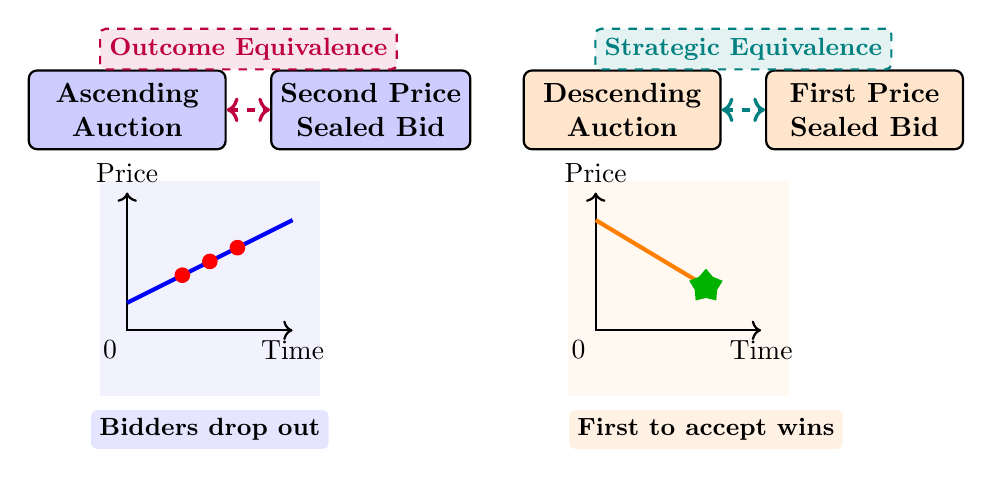
\begin{tikzpicture}[
    scale=0.7,
    auction/.style={
        rectangle,
        rounded corners=3pt,
        draw=black,
        thick,
        minimum width=2.5cm,
        minimum height=1cm,
        align=center,
        font=\bfseries
    },
    equiv/.style={
        rectangle,
        rounded corners=2pt,
        fill=white,
        draw=none,
        font=\small\bfseries
    }
]
    % TOP ROW Auction Types
    \node[auction, fill=blue!20] (eng_box) at (0, 0) {Ascending\\Auction};
    \node[auction, fill=blue!20, right=0.55cm of eng_box] (vickrey_box) {Second Price\\Sealed Bid};
    \node[auction, fill=orange!20, right=0.65cm of vickrey_box] (dutch_box) {Descending\\Auction};
    \node[auction, fill=orange!20, right=0.55cm of dutch_box] (firstprice_box) {First Price\\Sealed Bid};
    
    % Equivalence arrows
    \draw[dashed, <->, line width=1.2pt, purple] (eng_box.east) -- (vickrey_box.west) 
        node[midway, above=0.5cm, equiv, fill=purple!10, draw=purple, thick] {Outcome Equivalence};
    
    \draw[dashed, <->, line width=1.2pt, teal] (dutch_box.east) -- (firstprice_box.west) 
        node[midway, above=0.5cm, equiv, fill=teal!10, draw=teal, thick] {Strategic Equivalence};
    
    % Graphs
    \begin{scope}[shift={(0, -4)}]
        \fill[blue!5] (-0.5, -1.2) rectangle (3.5, 2.7);
        \draw[thick, ->] (0, 2) -- (0, 0) node[below left] {0} -- (3, 0) node[below] {Time};
        \draw[thick, ->] (0, 0) -- (0, 2.5) node[above] {Price};
        \draw[thick, blue, line width=1.5pt] (0, 0.5) -- (1, 1) -- (2, 1.5) -- (3, 2);
        \foreach \x in {1, 1.5, 2} {
            \node[circle, fill=red, inner sep=2pt] at (\x, {0.5 + 0.5*\x}) {};
        }
        \node[font=\small\bfseries, fill=blue!10, rounded corners=2pt, inner sep=3pt] at (1.5, -1.8) {Bidders drop out};
    \end{scope}
    
    \begin{scope}[shift={(8.5, -4)}]
        \fill[orange!5] (-0.5, -1.2) rectangle (3.5, 2.7);
        \draw[thick, ->] (0, 2) -- (0, 0) node[below left] {0} -- (3, 0) node[below] {Time};
        \draw[thick, ->] (0, 0) -- (0, 2.5) node[above] {Price};
        \draw[thick, orange, line width=1.5pt] (0, 2) -- (2, 0.8);
        \node[star, star points=5, fill=green!70!black, inner sep=3pt] at (2, 0.8) {};
        \node[font=\small\bfseries, fill=orange!10, rounded corners=2pt, inner sep=3pt] at (2, -1.8) {First to accept wins};
    \end{scope}
\end{tikzpicture}
\end{frame}


%===============================================
\section{Revenue Equivalence}
\sectionslide
%===============================================
\begin{frame}{Revenue Equivalence: The Surprising Result}
All six standard formats generate the same expected revenue!

\centering
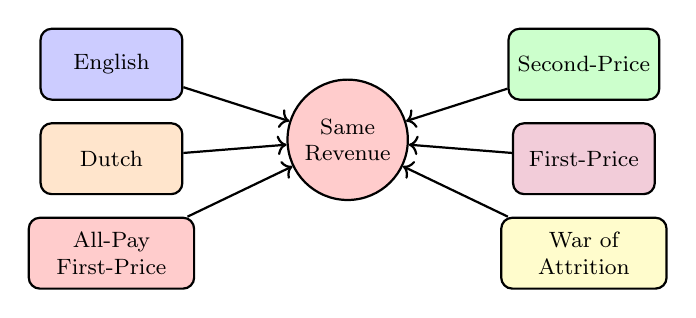
\begin{tikzpicture}[scale=0.8, every node/.style={draw, thick, rounded corners, font=\footnotesize, align=center}]
  % Six auction boxes
  \node[fill=blue!20, minimum width=1.8cm, minimum height=0.9cm] (eng)   at (-3.5,1.5) {English};
  \node[fill=green!20, minimum width=1.8cm, minimum height=0.9cm] (vick)  at (4,1.5) {Second-Price};
  \node[fill=orange!20, minimum width=1.8cm, minimum height=0.9cm] (dutch) at (-3.5,0)   {Dutch};
  \node[fill=purple!20, minimum width=1.8cm, minimum height=0.9cm] (first) at (4,0)   {First-Price};
  \node[fill=red!20, minimum width=2.1cm, minimum height=0.9cm]    (allpay) at (-3.5,-1.5) {All-Pay\\First-Price};
  \node[fill=yellow!20, minimum width=2.1cm, minimum height=0.9cm] (woa)   at (4,-1.5) {War of\\Attrition};

  % Revenue
  \node[draw, circle, thick, fill=red!20, minimum size=1.4cm] (rev) at (0.25,0.3) {Same\\Revenue};

  % Arrows
  \draw[->, thick] (eng)   -- (rev);
  \draw[->, thick] (vick)  -- (rev);
  \draw[->, thick] (dutch) -- (rev);
  \draw[->, thick] (first) -- (rev);
  \draw[->, thick] (allpay) -- (rev);
  \draw[->, thick] (woa)   -- (rev);
\end{tikzpicture}

\vspace{0.3em}
\textbf{Conditions Required:}
\begin{itemize}
  \item Independent private values (IPV); risk-neutral bidders
  \item Symmetric bidders (same distribution $F$); no collusion
\end{itemize}
\textbf{Key Insight:} Revenue determined by competition level, not payment rule
\end{frame}

\begin{frame}{Summary: Bid Functions and Revenue (Uniform $[0,1]$)}
\begin{center}
\begin{tabular}{lcc}
\toprule
\textbf{Format} & \textbf{Equilibrium Bid} $B(v)$ & \textbf{Revenue} \\
\midrule
English & $v$ & $\frac{n-1}{n+1}$ \\[0.2cm]
Second-Price & $v$ & $\frac{n-1}{n+1}$ \\[0.2cm]
First-Price & $\frac{n-1}{n}v$ & $\frac{n-1}{n+1}$ \\[0.2cm]
Dutch & $\frac{n-1}{n}v$ & $\frac{n-1}{n+1}$ \\[0.2cm]
All-Pay 1st & $\frac{n-1}{n}v^n$ & $\frac{n-1}{n+1}$ \\[0.2cm]
War of Attrition & $v + (1-v)\ln(1-v)$ & $\frac{n-1}{n+1}$ \\
& (for $n=2$) & \\
\bottomrule
\end{tabular}
\end{center}
\textbf{Key Observation:} All yield expected revenue = $\E[v_{(n-1)}] = \frac{n-1}{n+1}$
\end{frame}

\begin{frame}{Revenue Equivalence: The Big Picture}
\textbf{Central Question:} Which auction format generates the most revenue?

\textbf{Surprising Answer:} Under standard assumptions, \emph{all} standard auctions yield the same expected revenue!

\textbf{Standard Assumptions:}
\begin{itemize}
  \item Independent Private Values (IPV)
  \item Risk-neutral bidders
  \item Symmetric bidders (same distribution $F$)
  \item Efficient allocation (highest value wins)
  \item Zero payment for lowest type
\end{itemize}

\textbf{Implication:} Revenue differences come from \emph{violations} of these assumptions
\end{frame}

\begin{frame}{Revenue Equivalence Theorem}
\begin{theorem}[Revenue Equivalence --- Vickrey 1961, Myerson 1981]
Consider any two auction mechanisms satisfying:
\begin{enumerate}
  \item Same allocation rule (highest value wins)
  \item Same expected payment for lowest type ($\underline{v}$ pays 0)
\end{enumerate}
Then under IPV, risk neutrality, and symmetry, both mechanisms yield identical expected revenue.
\end{theorem}

All yield expected revenue = $\E[v_{(n-1)}]$
\end{frame}

\begin{frame}{Revenue Equivalence: Proof Sketch (1/2)}
\begin{proofbox}[Step 1: Expected Utility]
Bidder with value $v$ in equilibrium receives:
$U(v) = Q(v) \cdot v - M(v)$

where $Q(v) = $ probability of winning, $M(v) = $ expected payment

\textbf{Envelope Theorem:} $\frac{dU}{dv} = Q(v)$

Integrating from $\underline{v}$ to $v$:
$U(v) = U(\underline{v}) + \int_{\underline{v}}^{v} Q(t) \, dt$
\end{proofbox}

\textbf{Key Insight:} Expected utility depends only on $Q(\cdot)$ and $U(\underline{v})$
\end{frame}

\begin{frame}{Revenue Equivalence: Proof Sketch (2/2)}
\begin{proofbox}[Step 2: Expected Payment]
From $U(v) = Q(v) \cdot v - M(v)$:
$M(v) = Q(v) \cdot v - U(v) = Q(v) \cdot v - U(\underline{v}) - \int_{\underline{v}}^{v} Q(t) \, dt$

\textbf{Expected Revenue:}
$ER = n \cdot \E[M(v)] = n \cdot \int_{\underline{v}}^{\bar{v}} M(v) f(v) dv$

After integration by parts:
$ER = \E\left[\sum_i Q_i(v) \cdot \left(v_i - \frac{1-F(v_i)}{f(v_i)}\right)\right] - n \cdot U(\underline{v})$
\end{proofbox}

\textbf{Conclusion:} Revenue depends only on $Q(\cdot)$ and $U(\underline{v})$. Same allocation + same boundary condition $\Rightarrow$ same revenue!
\end{frame}

\begin{frame}{Revenue Equivalence: Verification}
\textbf{First-Price Auction} (Uniform $[0,1]$, $n$ bidders):

Equilibrium bid: $b(v) = \frac{n-1}{n}v$

Expected revenue: $\E[\text{highest bid}] = \E\left[\frac{n-1}{n}v_{(n)}\right] = \frac{n-1}{n} \cdot \frac{n}{n+1} = \frac{n-1}{n+1}$

\textbf{Second-Price Auction:}

Expected revenue: $\E[v_{(n-1)}] = \frac{n-1}{n+1}$ \checkmark

\textbf{All-Pay Auction:}

Expected total payments: $n \cdot \E\left[\frac{n-1}{n}v^n\right] = (n-1) \cdot \frac{1}{n+1} = \frac{n-1}{n+1}$ \checkmark
\end{frame}



\begin{frame}{What Revenue Equivalence Does NOT Say}
\textbf{Common Misconceptions:}

\begin{enumerate}
  \item ``All auctions are the same'' --- \textcolor{red}{False}
  \begin{itemize}
    \item Revenue equivalent $\neq$ strategically equivalent
    \item Bidding strategies differ dramatically
  \end{itemize}
  
  \item ``Revenue always equals $\E[v_{(n-1)}]$'' --- \textcolor{red}{False}
  \begin{itemize}
    \item Only for efficient mechanisms with $U(\underline{v}) = 0$
    \item Reserve prices change this
  \end{itemize}
  
  \item ``Real auctions satisfy revenue equivalence'' --- \textcolor{red}{Rarely}
  \begin{itemize}
    \item Risk aversion breaks it
    \item Common values break it
    \item Asymmetry breaks it
    \item Entry effects break it
  \end{itemize}
\end{enumerate}
\end{frame}



%===============================================
\section{Optimal Reserve Prices}
\sectionslide
%===============================================

\begin{frame}{Why Set a Reserve Price?}
\textbf{The Seller's Dilemma:}
\begin{itemize}
  \item Low reserve: More likely to sell, but possibly at low price
  \item High reserve: Higher conditional price, but risk no sale
\end{itemize}

\textbf{Key Insight:} Reserve price acts like an additional ``phantom bidder''

\textbf{Trade-off:}
\begin{center}
\begin{tikzpicture}[scale=0.8]
  \draw[->] (0,0) -- (6,0) node[right] {Reserve $r$};
  \draw[->] (0,0) -- (0,4) node[above] {Revenue};
  
  \draw[thick, blue, domain=0:4, samples=50] plot (\x, {3 - 0.5*(\x-2)^2 + 0.5});
  
  \node[red, fill=white] at (2,3.5) {$r^*$};
  \draw[red, dashed] (2,0) -- (2,3.5);
  \draw[red, fill=red] (2,3.5) circle (2pt);
  
  \node[below, font=\footnotesize] at (1,0) {Low};
  \node[below, font=\footnotesize] at (4,0) {High};
\end{tikzpicture}
\end{center}
\end{frame}

\begin{frame}{Optimal Reserve Price Formula}
\begin{theorem}[Myerson 1981]
The optimal reserve price $r^*$ satisfies:
$$r^* - \frac{1-F(r^*)}{f(r^*)} = v_s$$
where $v_s$ is the seller's valuation for the item.
\end{theorem}

\textbf{If seller values item at $v_s = 0$:}
$$r^* = \frac{1-F(r^*)}{f(r^*)}$$

\textbf{Interpretation:} Set reserve where ``virtual valuation'' equals seller's value

\textbf{Virtual Valuation:} $\psi(v) = v - \frac{1-F(v)}{f(v)}$

Reserve screens out bidders with negative virtual valuations
\end{frame}

\begin{frame}{Optimal Reserve: Uniform Example}
\textbf{Setup:} $v \sim U[0,1]$, seller value $v_s = 0$

\begin{proofbox}[Derivation]
$F(v) = v$, $f(v) = 1$

Optimal reserve condition: $r^* = \frac{1-r^*}{1} = 1 - r^*$

Solving: $2r^* = 1$ $\Rightarrow$ $\boxed{r^* = \frac{1}{2}}$
\end{proofbox}

\textbf{Key Results:}
\begin{itemize}
  \item Optimal reserve is \textbf{independent of $n$}!
  \item With 2 bidders: $r^* = 0.5$
  \item With 100 bidders: $r^* = 0.5$
  \item More bidders $\Rightarrow$ reserve less likely to bind
\end{itemize}
\end{frame}

\begin{frame}{Reserve Price: Revenue Impact}
\begin{center}
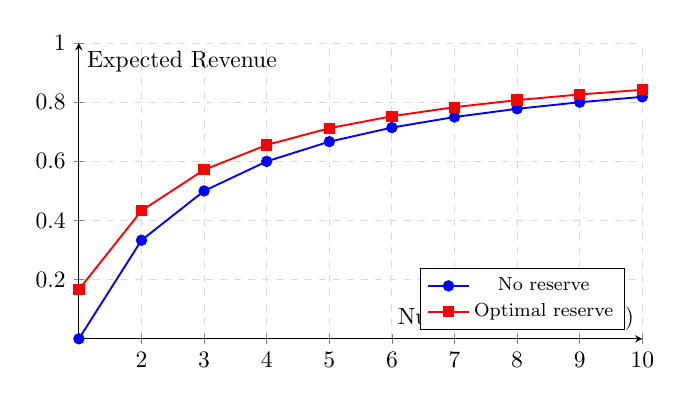
\begin{tikzpicture}[scale=0.85]
  \begin{axis}[
    xlabel={Number of Bidders ($n$)},
    ylabel={Expected Revenue},
    xmin=1, xmax=10,
    ymin=0, ymax=1,
    axis lines=middle,
    width=10cm,
    height=6cm,
    grid=major,
    grid style={dashed, gray!30},
    xtick={1,2,3,4,5,6,7,8,9,10},
    ytick={0,0.2,0.4,0.6,0.8,1},
    legend pos=south east,
    legend style={font=\footnotesize}
  ]
  
  % No reserve: E[v_(n-1)] = (n-1)/(n+1)
  \addplot[domain=1:10, samples=10, thick, blue, mark=*] {(x-1)/(x+1)};
  \addlegendentry{No reserve}
  
  % With optimal reserve (approximate formula for uniform)
  \addplot[domain=1:10, samples=10, thick, red, mark=square*] {(x-1)/(x+1) + 0.25/(x+0.5)};
  \addlegendentry{Optimal reserve}
  
  \end{axis}
\end{tikzpicture}
\end{center}

\textbf{Insight:} Reserve price benefit largest with few bidders
\end{frame}


\begin{frame}{Why Reserve Prices Matter}
\textbf{Reserve Price = Minimum acceptable bid}

\begin{center}
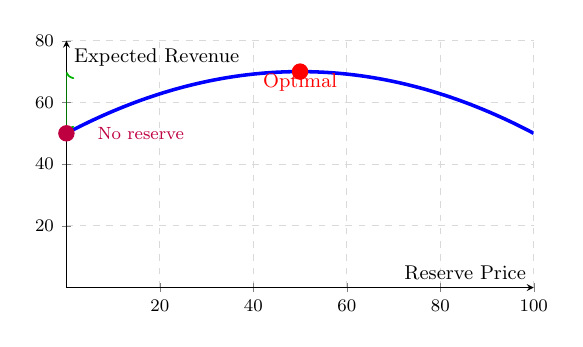
\begin{tikzpicture}[scale=0.80]
  \begin{axis}[
    xlabel={Reserve Price},
    ylabel={Expected Revenue},
    xmin=0, xmax=100,
    ymin=0, ymax=80,
    axis lines=middle,
    width=9cm,
    height=5.5cm,
    grid=major,
    grid style={dashed, gray!30},
    xtick={0,20,40,60,80,100},
    ytick={0,20,40,60,80},
    xlabel style={font=\small},
    ylabel style={font=\small},
    tick label style={font=\footnotesize}
  ]
  
  % Revenue curve
  \addplot[domain=0:100, samples=100, ultra thick, blue] {-0.008*(x-50)^2 + 70};
  
  % Optimal point
  \addplot[mark=*, mark size=3.5pt, only marks, red] coordinates {(50,70)};
  \node[below, red, font=\small] at (axis cs:50,72) {Optimal};
  
  % No reserve
  \addplot[mark=*, mark size=3.5pt, only marks, purple] coordinates {(0,50)};
  \node[right, purple, font=\footnotesize] at (axis cs:5,50) {No reserve};
  
  % Arrow showing gain
  \draw[<->, thick, green!70!black] (axis cs:0,50) -- (axis cs:0,70);
  \node[left, green!70!black, font=\footnotesize] at (axis cs:0,60) {+40\%};
  
  \end{axis}
\end{tikzpicture}
\end{center}

\textbf{Why They Work:}
\begin{itemize}
  \item Forces bidders to compete more aggressively
  \item Protects against low-ball bids
  \item Trade-off: Higher revenue vs. probability of no sale
  \item New Zealand spectrum disaster: no reserve = \$1 winning bid!
\end{itemize}
\end{frame}


\begin{frame}{Virtual Valuation Illustration}
\begin{center}
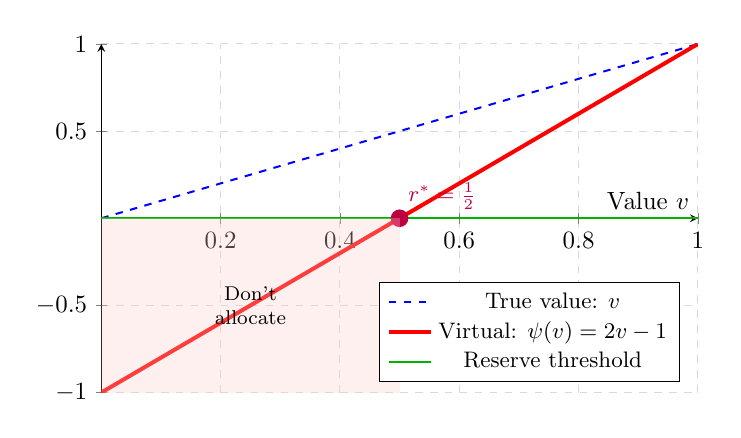
\begin{tikzpicture}[scale=0.9]
  \begin{axis}[
    xlabel={Value $v$},
    ylabel={},
    xmin=0, xmax=1,
    ymin=-1, ymax=1,
    axis lines=middle,
    legend pos=south east,
    legend style={font=\small},
    width=10cm,
    height=6.5cm,
    grid=major,
    grid style={dashed, gray!30}
  ]
  
  % 45-degree line (true value)
  \addplot[domain=0:1, thick, dashed, blue] {x};
  \addlegendentry{True value: $v$}
  
  % Virtual valuation
  \addplot[domain=0:1, ultra thick, red] {2*x - 1};
  \addlegendentry{Virtual: $\psi(v) = 2v-1$}
  
  % Zero line
  \addplot[domain=0:1, thick, green!70!black] {0};
  \addlegendentry{Reserve threshold}
  
  % Intersection
  \node[circle, fill=purple, inner sep=2.5pt] at (axis cs:0.5,0) {};
  \node[above right, purple, font=\small] at (axis cs:0.5,0) {$r^* = \frac{1}{2}$};
  
  % Shading
  \fill[red!20, opacity=0.3] (axis cs:0,-1) rectangle (axis cs:0.5,0);
  \node[align=center, font=\footnotesize] at (axis cs:0.25,-0.5) {Don't\\allocate};
  
  \end{axis}
\end{tikzpicture}
\end{center}

\textbf{Key:} Allocate only when $\psi(v) \geq 0$ (or $\geq v_s$ if seller has value)
\end{frame}

\begin{frame}{Reserve Price: Practical Considerations}
\textbf{When to Use High Reserve:}
\begin{itemize}
  \item Few bidders expected
  \item Seller has high value for keeping item
  \item Can re-auction later if no sale
\end{itemize}

\textbf{When to Use Low/No Reserve:}
\begin{itemize}
  \item Many bidders expected
  \item Perishable goods (time-sensitive)
  \item Reputation concerns (commitment to sell)
\end{itemize}

\textbf{Secret vs. Public Reserve:}
\begin{itemize}
  \item Public reserve: Transparent, builds trust
  \item Secret reserve: Can adjust based on bidding
  \item Empirically: Public reserves often perform better
\end{itemize}
\end{frame}

%===============================================
\section{Entry and Participation}
\sectionslide
%===============================================

\begin{frame}{The Entry Problem}
\textbf{Standard Theory Assumes:} Fixed number of bidders $n$

\textbf{Reality:} Bidders choose whether to participate

\textbf{Entry Decision:}
\begin{itemize}
  \item Entry cost: $c > 0$ (time, preparation, due diligence)
  \item Expected profit from participating: $\E[\pi | \text{enter}]$
  \item Enter if: $\E[\pi | \text{enter}] \geq c$
\end{itemize}

\textbf{Implications:}
\begin{itemize}
  \item Entry is endogenous
  \item Auction format affects entry
  \item Revenue equivalence may break down
\end{itemize}
\end{frame}

\begin{frame}{Entry: Free Entry Equilibrium}
\textbf{Free Entry Condition:}
$$\E[\text{profit} | n \text{ entrants}] = c$$

\textbf{With Symmetric IPV:}

For first-price auction with $v \sim U[0,1]$:
$$\E[\pi] = \int_0^1 \frac{v^n}{n} dv = \frac{1}{n(n+1)}$$

Free entry: $\frac{1}{n^*(n^*+1)} = c$ $\Rightarrow$ $n^* \approx \frac{1}{\sqrt{c}}$

\textbf{Key Result:} Higher entry cost $\Rightarrow$ fewer bidders $\Rightarrow$ lower revenue
\end{frame}



\begin{frame}{Entry and Information Acquisition}
\begin{center}
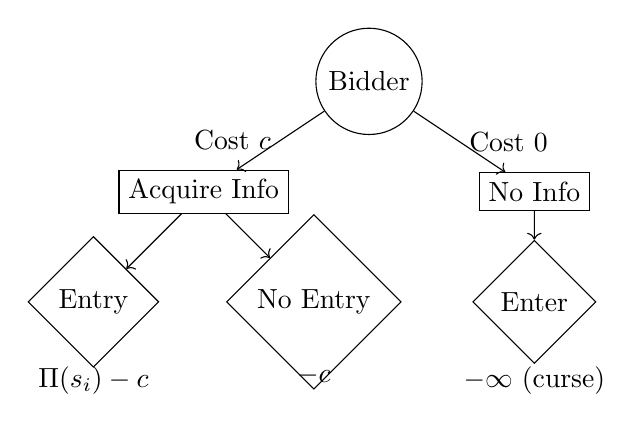
\begin{tikzpicture}[scale=0.7]
  % Decision tree
  \node[draw, circle] (start) at (0,0) {Bidder};
  \node[draw, rectangle] (acquire) at (-3,-2) {Acquire Info};
  \node[draw, rectangle] (noinfo) at (3,-2) {No Info};
  
  \draw[->] (start) -- (acquire) node[midway,left] {Cost $c$};
  \draw[->] (start) -- (noinfo) node[midway,right] {Cost $0$};
  
  \node[draw, diamond] (enter1) at (-5,-4) {Entry};
  \node[draw, diamond] (nenter1) at (-1,-4) {No Entry};
  \node[draw, diamond] (enter2) at (3,-4) {Enter};
  
  \draw[->] (acquire) -- (enter1);
  \draw[->] (acquire) -- (nenter1);
  \draw[->] (noinfo) -- (enter2);
  
  % Payoffs
  \node[below] at (-5,-5) {$\Pi(s_i) - c$};
  \node[below] at (-1,-5) {$-c$};
  \node[below] at (3,-5) {$-\infty$ (curse)};
\end{tikzpicture}
\end{center}

\textbf{Equilibrium Effects:}
\begin{itemize}
  \item Information acquisition creates entry barrier; Uninformed bidders face winner's curse
  \item Can lead to thin markets/breakdown; English auctions partially mitigate through revelation
\end{itemize}
\end{frame}


\begin{frame}{Entry vs. Information Effects}
\begin{center}
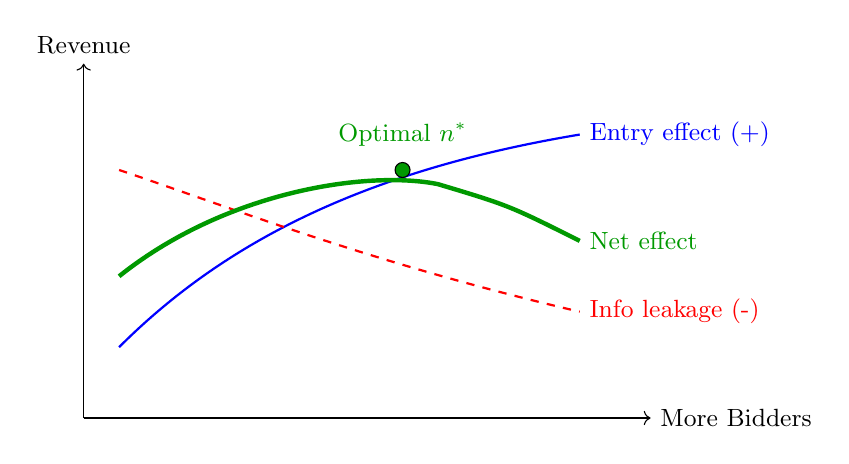
\begin{tikzpicture}[scale=0.9]
  % Draw axes
  \draw[->] (0,0) -- (8,0) node[right] {\small More Bidders};
  \draw[->] (0,0) -- (0,5) node[above] {\small Revenue};
  
  % Entry effect (solid blue, increasing)
  \draw[thick, blue] (0.5,1) .. controls (2,2.5) and (4,3.5) .. (7,4);
  \node[blue, right, font=\small] at (7,4) {Entry effect (+)};
  
  % Information effect (dashed red, potentially decreasing for common values)
  \draw[thick, red, dashed] (0.5,3.5) .. controls (2,3) and (4,2.2) .. (7,1.5);
  \node[red, right, font=\small] at (7,1.5) {Info leakage (-)};
  
  % Net effect (green, hump-shaped)
  \draw[ultra thick, green!60!black] (0.5,2) .. controls (2,3.2) and (4,3.5) .. (5,3.3) .. controls (6,3) .. (7,2.5);
  \node[green!60!black, right, font=\small] at (7,2.5) {Net effect};
  
  % Optimal point
  \draw[fill=green!60!black] (4.5,3.5) circle (3pt);
  \node[above, green!60!black, font=\small] at (4.5,3.7) {Optimal $n^*$};
\end{tikzpicture}
\end{center}

\textbf{Trade-off:}
\begin{itemize}
  \item More bidders $\rightarrow$ more competition $\rightarrow$ higher prices
  \item More bidders $\rightarrow$ more information revealed $\rightarrow$ winner's curse
\end{itemize}
\end{frame}

\begin{frame}{Auction Format and Entry}
\begin{center}
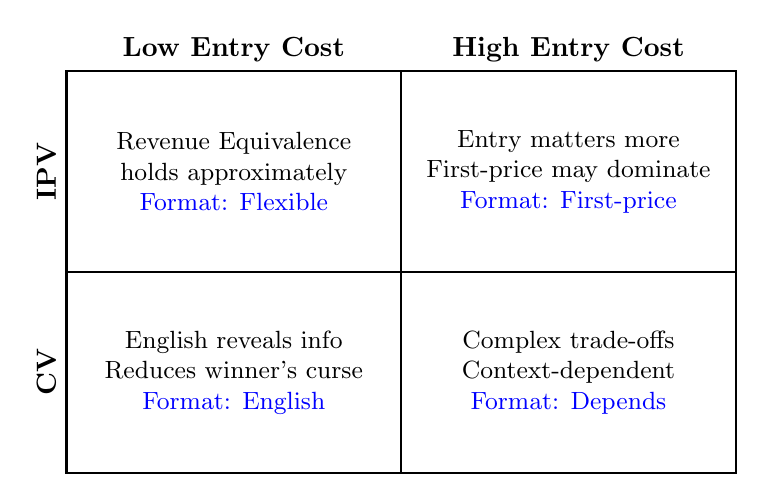
\begin{tikzpicture}[scale=0.85]
  % Create a 2x2 grid
  \draw[thick] (0,0) rectangle (10,6);
  \draw[thick] (5,0) -- (5,6);
  \draw[thick] (0,3) -- (10,3);
  
  % Labels
  \node[above, font=\bfseries] at (2.5,6) {Low Entry Cost};
  \node[above, font=\bfseries] at (7.5,6) {High Entry Cost};
  \node[left, font=\bfseries, rotate=90, anchor=center] at (-0.3,4.5) {IPV};
  \node[left, font=\bfseries, rotate=90, anchor=center] at (-0.3,1.5) {CV};
  
  % Content - Top Left (IPV, Low Cost)
  \node[align=center, font=\small] at (2.5,4.5) {Revenue Equivalence\\holds approximately\\{\color{blue}Format: Flexible}};
  
  % Content - Top Right (IPV, High Cost)
  \node[align=center, font=\small] at (7.5,4.5) {Entry matters more\\First-price may dominate\\{\color{blue}Format: First-price}};
  
  % Content - Bottom Left (CV, Low Cost)
  \node[align=center, font=\small] at (2.5,1.5) {English reveals info\\Reduces winner's curse\\{\color{blue}Format: English}};
  
  % Content - Bottom Right (CV, High Cost)  
  \node[align=center, font=\small] at (7.5,1.5) {Complex trade-offs\\Context-dependent\\{\color{blue}Format: Depends}};
\end{tikzpicture}
\end{center}
\end{frame}

%===============================================
\section{Optimal Auction Design}
\sectionslide
%===============================================

\begin{frame}{The Optimal Auction Problem}
\textbf{Seller's Goal:} Design mechanism to maximize expected revenue

\textbf{Constraints:}
\begin{itemize}
  \item Incentive Compatibility (IC): Truth-telling is optimal
  \item Individual Rationality (IR): Bidders willing to participate
\end{itemize}

\textbf{Myerson's Approach:}
\begin{enumerate}
  \item Use Revelation Principle: Focus on direct mechanisms
  \item Characterize IC constraints
  \item Optimize over feasible mechanisms
\end{enumerate}
\end{frame}

\begin{frame}{Virtual Valuations}
\begin{definition}[Virtual Valuation]
$$\psi(v) = v - \frac{1-F(v)}{f(v)}$$
\end{definition}

\textbf{Interpretation:}
\begin{itemize}
  \item $v$ = bidder's actual value
  \item $\frac{1-F(v)}{f(v)}$ = information rent given to higher types
  \item $\psi(v)$ = marginal revenue from serving type $v$
\end{itemize}

\textbf{Regularity Condition:} $\psi(v)$ increasing in $v$

\begin{alertblock}{Key Result}
Expected revenue = $\E[\psi(v) \cdot \mathbf{1}_{\text{win}}]$

To maximize revenue: allocate to bidder with highest $\psi(v_i) \geq 0$
\end{alertblock}
\end{frame}

\begin{frame}{Myerson's Optimal Auction}
\begin{theorem}[Myerson 1981]
The optimal auction allocates to the bidder with highest virtual valuation, provided it exceeds zero.
\end{theorem}

\textbf{Implementation:}
\begin{enumerate}
  \item Compute virtual valuations $\psi_i(v_i)$ for all bidders
  \item Allocate to $i^* = \argmax_i \psi_i(v_i)$ if $\psi_{i^*} \geq 0$
  \item Charge payment that makes truth-telling optimal
\end{enumerate}

\textbf{For Symmetric Regular Distributions:}
\begin{itemize}
  \item Optimal auction = Second-price with optimal reserve $r^*$
  \item Reserve satisfies $\psi(r^*) = 0$
\end{itemize}
\end{frame}

\begin{frame}{Optimal Auction: Uniform Example}
\textbf{Setup:} $n=2$ bidders, $v_i \sim U[0,1]$

\textbf{Virtual Valuation:} $\psi(v) = v - \frac{1-v}{1} = 2v - 1$

\textbf{Optimal Reserve:} $\psi(r^*) = 0$ $\Rightarrow$ $2r^* - 1 = 0$ $\Rightarrow$ $r^* = \frac{1}{2}$

\begin{proofbox}[Revenue Comparison]
\textbf{Without reserve:}
$ER = \E[v_{(1)}] = \frac{1}{3}$

\textbf{With optimal reserve $r^* = 0.5$:}
$ER = \frac{1}{3} + \frac{1}{2} \cdot P(\text{both} < 0.5) \cdot 0.5 = \frac{1}{3} + \frac{1}{8} = \frac{11}{24} \approx 0.458$

\textbf{Revenue gain:} $\frac{11/24 - 1/3}{1/3} = 37.5\%$
\end{proofbox}
\end{frame}

\begin{frame}{Beyond Standard Optimal Auctions}
\textbf{Asymmetric Bidders:}
\begin{itemize}
  \item Different distributions $F_i$ for each bidder
  \item Optimal auction may favor ``weaker'' bidders
  \item Discriminatory reserve prices possible
\end{itemize}

\textbf{Risk-Averse Bidders:}
\begin{itemize}
  \item First-price $>$ second-price revenue
  \item Optimal auction exploits risk aversion
\end{itemize}

\textbf{Correlated Values:}
\begin{itemize}
  \item Crémer-McLean mechanism can extract full surplus
  \item Relies on ability to correlate payments with others' reports
  \item Fragile to collusion and model misspecification
\end{itemize}
\end{frame}

%===============================================
\section{Strategic Equivalences}
\sectionslide
%===============================================

\begin{frame}{Strategic vs. Revenue Equivalence}
\begin{center}
\begin{tabular}{lcc}
\toprule
\textbf{Auction Pair} & \textbf{Strategic Eq.} & \textbf{Revenue Eq.} \\
\midrule
English vs. Second-Price & IPV only & Yes \\
Dutch vs. First-Price & \textcolor{green!70!black}{Always} & Yes \\
First-Price vs. Second-Price & No & IPV + RN \\
English vs. Dutch & No & IPV + RN \\
All-Pay vs. First-Price & No & IPV + RN \\
\bottomrule
\end{tabular}
\end{center}

\textbf{Strategic Equivalence:} Same strategies in equilibrium

\textbf{Revenue Equivalence:} Same expected revenue (weaker)
\end{frame}

\begin{frame}{The Equivalence Hierarchy}
\begin{center}
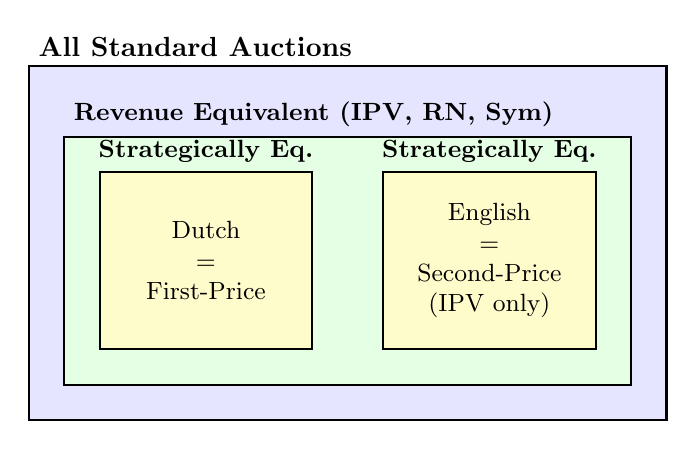
\begin{tikzpicture}[scale=0.9]
  % Draw nested boxes
  \draw[thick, fill=blue!10] (0,0) rectangle (9,5);
  \node[above right, font=\bfseries] at (0,5) {All Standard Auctions};
  
  \draw[thick, fill=green!10] (0.5,0.5) rectangle (8.5,4);
  \node[above right, font=\bfseries\small] at (0.5,4) {Revenue Equivalent (IPV, RN, Sym)};
  
  \draw[thick, fill=yellow!20] (1,1) rectangle (4,3.5);
  \node[above, font=\small\bfseries] at (2.5,3.5) {Strategically Eq.};
  \node[align=center, font=\small] at (2.5,2.25) {Dutch\\=\\First-Price};
  
  \draw[thick, fill=yellow!20] (5,1) rectangle (8,3.5);
  \node[above, font=\small\bfseries] at (6.5,3.5) {Strategically Eq.};
  \node[align=center, font=\small] at (6.5,2.25) {English\\=\\Second-Price\\(IPV only)};
\end{tikzpicture}
\end{center}
\end{frame}

\begin{frame}{Summary: Core Results}
\textbf{Revenue Equivalence:}
\begin{itemize}
  \item Under IPV + RN + Symmetry: All standard auctions yield same revenue
  \item Revenue = $\E[v_{(n-1)}]$ with efficient allocation
\end{itemize}

\textbf{Optimal Reserve:}
\begin{itemize}
  \item Set where virtual valuation = seller's value
  \item Independent of number of bidders
  \item Uniform $[0,1]$: $r^* = 0.5$
\end{itemize}

\textbf{Optimal Auction:}
\begin{itemize}
  \item Allocate to highest virtual valuation $\geq 0$
  \item For symmetric regular: Second-price + optimal reserve
\end{itemize}

\textbf{Entry:}
\begin{itemize}
  \item Endogenous participation affects format choice
  \item Trade-off between competition and information effects
\end{itemize}
\end{frame}


\part{Relaxing Assumptions}
\partslide
%===============================================
\begin{frame}{The Auction Trilemma: You Can't Have It All}
\textbf{The Three Desirable Properties}

\begin{center}
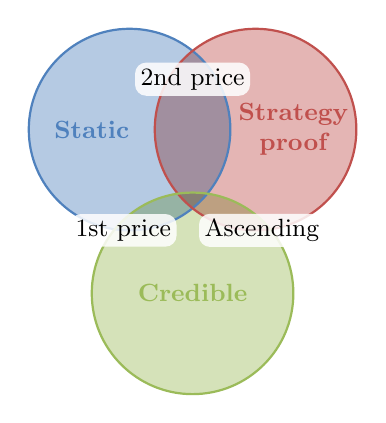
\begin{tikzpicture}[scale=1.6, every node/.style={font=\small}]
    % Define consistent colors
    \definecolor{staticcolor}{RGB}{79,129,189}
    \definecolor{stratproofcolor}{RGB}{192,80,77}
    \definecolor{crediblecolor}{RGB}{155,187,89}

    % Transparency layer
    \begin{scope}[blend group = multiply]
        \fill[staticcolor!60, opacity=0.7] (-0.5,0.8) circle (0.8cm);
        \fill[stratproofcolor!60, opacity=0.7] (0.5,0.8) circle (0.8cm);
        \fill[crediblecolor!60, opacity=0.7] (0,-0.5) circle (0.8cm);
    \end{scope}

    % Circle outlines
    \draw[thick, staticcolor] (-0.5,0.8) circle (0.8cm);
    \draw[thick, stratproofcolor] (0.5,0.8) circle (0.8cm);
    \draw[thick, crediblecolor] (0,-0.5) circle (0.8cm);

    % Labels for sets
    \node[font=\small\bfseries, staticcolor] at (-0.8,0.8) {Static};
    \node[font=\small\bfseries, stratproofcolor, align=center] at (0.8,0.8){Strategy\\proof};
    \node[font=\small\bfseries, crediblecolor] at (0,-0.5) {Credible};

    % Labels for intersections
    \node[align=center, fill=white, rounded corners, opacity=0.85, text opacity=1, inner sep=2pt]
        at (0,1.2) {2nd price};
    \node[align=center, fill=white, rounded corners, opacity=0.85, text opacity=1, inner sep=2pt]
        at (-0.55, 0) {1st price};
    \node[align=center, fill=white, rounded corners, opacity=0.85, text opacity=1, inner sep=2pt]
        at (0.55,0) {Ascending};
\end{tikzpicture}
\end{center}

\begin{itemize}
  \item \textbf{Static:} No time dimension, all decisions simultaneous
  \item \textbf{Strategy-proof:} Bidding true value is optimal
  \item \textbf{Credible:} Auctioneer cannot manipulate for higher revenue
\end{itemize}
\end{frame}

\section{Relaxing Risk Neutrality}

\begin{frame}{Relaxing Risk Neutrality}
\textbf{The Assumption:} Bidders maximize expected monetary value

\textbf{Reality:} Most bidders are risk-averse
\begin{itemize}
  \item Utility $U(x)$ is concave: $U''(x) < 0$
  \item Prefer certain \$50 over 50\% chance of \$100
\end{itemize}

\textbf{Impact on Standard Formats:}

\textbf{English \& Second-Price:} \textcolor{green!70!black}{No impact!}
\begin{itemize}
  \item Bidding true value still dominant
  \item Risk preferences irrelevant
  \item Revenue unchanged
\end{itemize}

\textbf{First-Price \& Dutch:} \textcolor{orange}{Higher bids!}
\begin{itemize}
  \item Risk-averse bidders bid closer to true value
  \item Trade certainty of winning for lower profit
  \item \textbf{Higher revenue for seller}
  \item Efficiency preserved
\end{itemize}
\end{frame}

\begin{frame}{Risk Aversion: Why Bid Higher in First-Price?}
\begin{center}
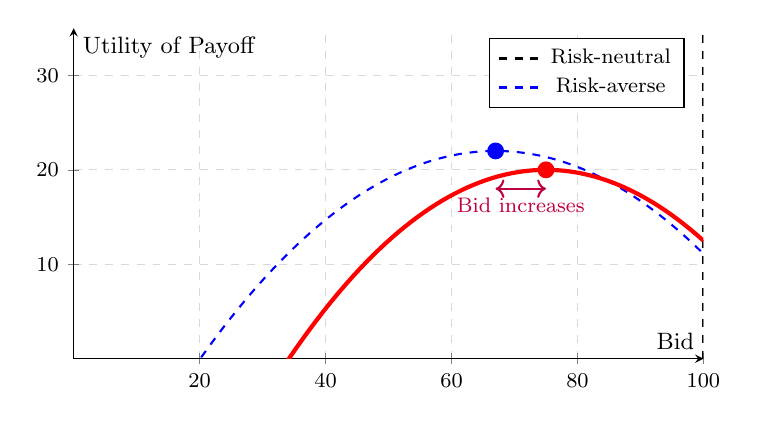
\begin{tikzpicture}[scale=0.95]
  \begin{axis}[
    xlabel={Bid},
    ylabel={Utility of Payoff},
    xmin=0, xmax=100,
    ymin=0, ymax=35,
    axis lines=middle,
    width=10cm,
    height=6cm,
    grid=major,
    grid style={dashed, gray!30},
    xlabel style={font=\small},
    ylabel style={font=\small},
    tick label style={font=\footnotesize},
    legend pos=north east,
    legend style={font=\footnotesize}
  ]
  
  % Value line
  \addplot[domain=0:100, samples=2, very thick, black, dashed] coordinates {(100,0) (100,35)};
  \node[font=\footnotesize] at (axis cs:100,37) {Value \$100K};
  
  % Risk-neutral curve
  \addplot[domain=0:100, samples=100, thick, blue, dashed] {-0.01*(x-67)^2 + 22};
  \addlegendentry{Risk-neutral}
  
  % Risk-averse curve
  \addplot[domain=0:100, samples=100, ultra thick, red] {-0.012*(x-75)^2 + 20};
  \addlegendentry{Risk-averse}
  
  % Optimal bids
  \addplot[mark=*, mark size=3pt, only marks, blue] coordinates {(67,22)};
  \addplot[mark=*, mark size=3pt, only marks, red] coordinates {(75,20)};
  
  % Arrow
  \draw[<->, thick, purple] (axis cs:67,18) -- (axis cs:75,18);
  \node[below, purple, font=\footnotesize] at (axis cs:71,18) {Bid increases};
  
  \end{axis}
\end{tikzpicture}
\end{center}

\textbf{Key Insight:} Risk aversion shifts optimal bid higher
\begin{itemize}
  \item Values certainty of winning
  \item Willing to sacrifice profit to increase win probability
\end{itemize}
\end{frame}

\begin{frame}{Risk Aversion: Revenue Rankings}
\textbf{Revenue Equivalence Breaks Down!}

\textbf{With Risk-Neutral Bidders:}
$$\text{First-Price Revenue} = \text{Second-Price Revenue} = \text{English Revenue}$$

\textbf{With Risk-Averse Bidders:}
$$\textcolor{red}{\textbf{First-Price Revenue} > \textbf{Second-Price Revenue} = \textbf{English Revenue}}$$

\textbf{Why:}
\begin{itemize}
  \item Second-price/English: Bidding true value still optimal
  \item First-price: Risk aversion increases bids
  \item \textbf{Practical implication:} Use first-price when bidders risk-averse
\end{itemize}

\textbf{Efficiency:}
\begin{itemize}
  \item \textcolor{green!70!black}{\textbf{Preserved in all formats!}}
  \item Highest-value bidder still wins
\end{itemize}
\end{frame}


\begin{frame}{All-Pay Auctions with Risk Aversion}
\textbf{The Dangerous Combination:} Risk aversion + pay even if you lose

\textbf{Strategic Effects:}
\begin{itemize}
  \item Risk-averse bidders \textit{extremely} conservative in all-pay auctions
  \item Two sources of risk:
  \begin{enumerate}
    \item Risk of losing and paying your bid (standard all-pay risk)
    \item Risk aversion amplifies the pain of losing
  \end{enumerate}
\end{itemize}


\begin{center}
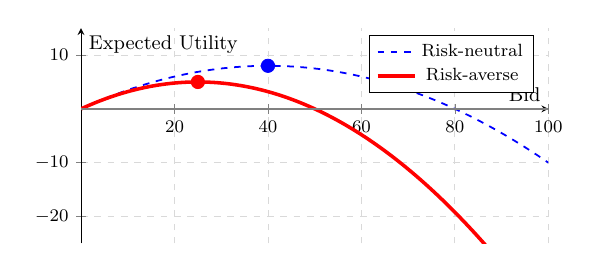
\begin{tikzpicture}[scale=0.8]
  \begin{axis}[
    xlabel={Bid},
    ylabel={Expected Utility},
    xmin=0, xmax=100,
    ymin=-25, ymax=15,
    axis lines=middle,
    width=9cm,
    height=5cm,
    grid=major,
    grid style={dashed, gray!30},
    xtick={0,20,40,60,80,100},
    ytick={-20,-10,0,10},
    xlabel style={font=\small},
    ylabel style={font=\small},
    tick label style={font=\footnotesize},
    legend pos=north east,
    legend style={font=\footnotesize}
  ]
  
  % Risk-neutral curve (from earlier slide)
  \addplot[domain=0:100, samples=100, thick, blue, dashed] {-0.005*(x-40)^2 + 8};
  \addlegendentry{Risk-neutral}
  
  % Risk-averse curve (peaks much earlier and lower)
  \addplot[domain=0:100, samples=100, ultra thick, red] {-0.008*(x-25)^2 + 5};
  \addlegendentry{Risk-averse}
  
  % Optimal bid markers
  \addplot[mark=*, mark size=3pt, only marks, blue] coordinates {(40,8)};
  \addplot[mark=*, mark size=3pt, only marks, red] coordinates {(25,5)};
  
  % Zero line
  \addplot[domain=0:100, samples=2, thick, gray] coordinates {(0,0) (100,0)};
  
  \end{axis}
\end{tikzpicture}
\end{center}

\textit{Risk aversion + all-pay = very low bidding and participation}
\end{frame}

\section{Relaxing Symmetry}

\begin{frame}{Asymmetric Bidders}
\textbf{The Assumption:} All bidders from same distribution $F(v)$

\textbf{Reality:} Different bidder types
\begin{itemize}
  \item Strong bidders: Values from $F_S(v)$
  \item Weak bidders: Values from $F_W(v)$
\end{itemize}

\textbf{Impact:}

\textbf{English \& Second-Price:} \textcolor{green!70!black}{No impact!}
\begin{itemize}
  \item Still dominant to bid true value
  \item Efficient allocation preserved
\end{itemize}

\textbf{First-Price \& Dutch:} \textcolor{red}{Major changes!}
\begin{itemize}
  \item Different equilibrium bid functions $B_i(v)$ per type
  \item \textbf{May lose efficiency}: Weak bidder with higher value may lose
  \item Revenue effects ambiguous
  \item Complex equilibrium
\end{itemize}
\end{frame}

\begin{frame}{Asymmetric Equilibrium Example}
\begin{center}
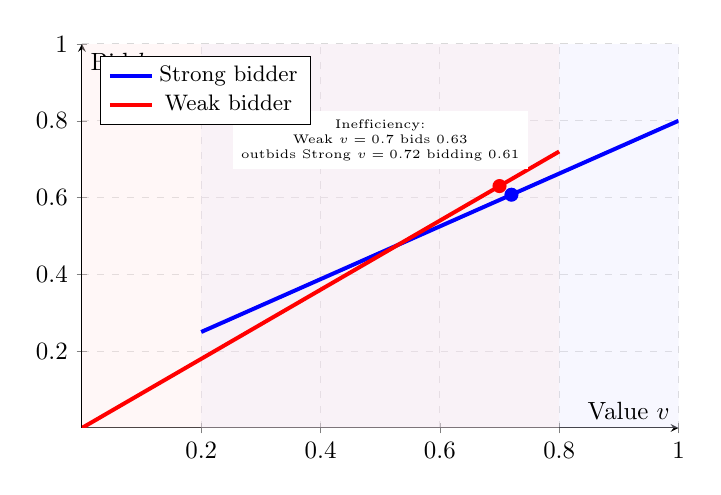
\begin{tikzpicture}[scale=0.9]
  \begin{axis}[
    xlabel={Value $v$},
    ylabel={Bid $b$},
    xmin=0, xmax=1,
    ymin=0, ymax=1,
    axis lines=middle,
    legend pos=north west,
    legend style={font=\small},
    width=10cm,
    height=7cm,
    grid=major,
    grid style={dashed, gray!30}
  ]
  
  % Support regions
  \fill[blue!10, opacity=0.3] (axis cs:0.2,0) rectangle (axis cs:1,1);
  \fill[red!10, opacity=0.3] (axis cs:0,0) rectangle (axis cs:0.8,1);
  
  % Bid functions
  \addplot[domain=0.2:1, ultra thick, blue] {0.6875*x + 0.1125};
  \addlegendentry{Strong bidder}
  
  \addplot[domain=0:0.8, ultra thick, red] {0.9*x};
  \addlegendentry{Weak bidder}
  
  % Inefficiency example
  \node[circle, fill=red, inner sep=2pt] at (axis cs:0.7,0.63) {};
  \node[circle, fill=blue, inner sep=2pt] at (axis cs:0.72,0.6075) {};
  
  \node[align=center, font=\tiny, fill=white] at (axis cs:0.5,0.75) {
    Inefficiency:\\
    Weak $v=0.7$ bids $0.63$\\
    outbids Strong $v=0.72$ bidding $0.61$
  };
  
  \end{axis}
\end{tikzpicture}
\end{center}

\textbf{Note:} Strong: $v \sim U[0.2,1]$, Weak: $v \sim U[0,0.8]$
\end{frame}

\section{Relaxing Independent Private Values}

\begin{frame}{Common Values and Winner's Curse}
\textbf{The Assumption:} Each bidder's value independent

\textbf{Reality:} Common Value situations
\begin{itemize}
  \item True value $V$ same for all
  \item Each has different signal/estimate $s_i$
  \item Example: Oil drilling rights
\end{itemize}

\textbf{The Winner's Curse:}
\begin{itemize}
  \item Winning means you had highest estimate
  \item If signals unbiased: $\E[S_i] = V$
  \item But: $\E[V | S_i = s, \text{Win}] < s$
  \item Naive bidding leads to losses!
\end{itemize}

\textbf{Rational Response:}
\begin{itemize}
  \item Account for adverse selection
  \item Bid conditional on being "just winning"
  \item Shade bid more with more competitors
\end{itemize}
\end{frame}

\begin{frame}{Visualizing the Winner's Curse}
\begin{center}
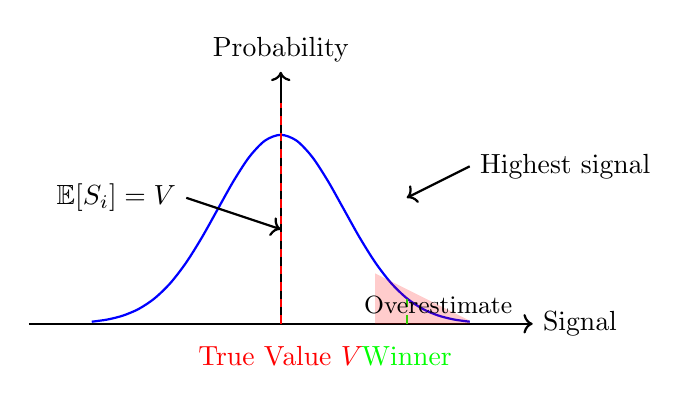
\begin{tikzpicture}[scale=0.8]
  % Draw normal distribution
  \draw[thick,->] (-4,0) -- (4,0) node[right] {Signal};
  \draw[thick,->] (0,0) -- (0,4) node[above] {Probability};
  
  % Bell curve
  \draw[thick,blue,domain=-3:3,smooth,variable=\x] plot ({\x},{3*exp(-\x*\x/2)});
  
  % True value
  \draw[thick,red,dashed] (0,0) -- (0,3.5);
  \node[below,red] at (0,-0.2) {True Value $V$};
  
  % Winner's signal
  \draw[thick,green,dashed] (2,0) -- (2,0.5);
  \node[below,green] at (2,-0.2) {Winner};
  
  % Annotations
  \draw[<-,thick] (2,2) -- (3,2.5) node[right] {Highest signal};
  \draw[<-,thick] (0,1.5) -- (-1.5,2) node[left] {$\E[S_i] = V$};
  
  % Shaded overestimate
  \fill[red,opacity=0.2] (1.5,0) -- (1.5,0.8) -- (3,0.05) -- (3,0) -- cycle;
  \node at (2.5,0.3) {\small Overestimate};
\end{tikzpicture}
\end{center}

\textbf{Lesson:} Winner has most optimistic signal, likely overestimate
\end{frame}

\begin{frame}{Impact on Formats: Common Values}
\textbf{English (Ascending):}
\begin{itemize}
  \item \textcolor{green!70!black}{\textbf{Advantage:}} Information revelation
  \item Bidders update beliefs as others drop out
  \item Reduces winner's curse
  \item More efficient information aggregation
\end{itemize}

\textbf{Sealed-Bid:}
\begin{itemize}
  \item \textcolor{red}{\textbf{Disadvantage:}} No information revelation
  \item Winner's curse more severe
  \item Aggressive bid shading
  \item Lower revenue
\end{itemize}

\textbf{Revenue Rankings:}
$$\text{English} > \text{First-Price} > \text{Second-Price}$$

\textbf{Key Result:} Revenue equivalence breaks down with common values
\end{frame}

\subsection{Linkage Principle}

\begin{frame}{Affiliated Values}
\textbf{Affiliation:} Random variables are affiliated if:
$$f(x \vee x') \cdot f(x \wedge x') \geq f(x) \cdot f(x')$$

\textbf{Intuition:}
\begin{itemize}
  \item Higher values of one variable make high values of others more likely
  \item Stronger than correlation
  \item Common in auctions
\end{itemize}

\textbf{Examples:}
\begin{itemize}
  \item Signals about common value
  \item Expert evaluations of artwork
  \item Geological surveys for oil
\end{itemize}
\end{frame}

\begin{frame}{The Linkage Principle}
\textbf{Milgrom-Weber Result:}

More information revelation $\Rightarrow$ Higher expected revenue

\textbf{Revenue Ranking with Affiliation:}
$$R_{English} \geq R_{Second-Price} \geq R_{First-Price}$$

\textbf{Why:}
\begin{itemize}
  \item English: Progressive information revelation
  \item Second-price: Winner learns second-highest bid
  \item First-price: No information revelation
\end{itemize}

\textbf{Policy Implication:}
\begin{itemize}
  \item Sellers should reveal information
  \item Public reserve better than secret reserve
  \item Provide inspection opportunities
\end{itemize}
\end{frame}

\section{Entry and Participation Costs}

\begin{frame}{Entry Costs in Auctions}
\textbf{Reality:} Participating in auctions is costly
\begin{itemize}
  \item Due diligence and valuation
  \item Legal and consulting fees
  \item Opportunity cost of time
  \item Bid preparation
\end{itemize}

\textbf{Impact:}
\begin{itemize}
  \item Fewer bidders enter than total pool
  \item Entry decision is strategic
  \item Affects competition and revenue
  \item May want to subsidize entry
\end{itemize}

\textbf{Key Questions:}
\begin{enumerate}
  \item How many bidders will enter?
  \item Should seller charge/subsidize entry?
  \item How does entry cost affect format choice?
\end{enumerate}
\end{frame}

\begin{frame}{Endogenous Entry Model (Levin-Smith 1994)}
\begin{itemize}
  \item Values: $v_i \sim F[0,1]$ revealed after entry
  \item Sequential: Entry $\rightarrow$ Learn value $\rightarrow$ Bid
\end{itemize}

\textbf{Entry Decision:}
\begin{itemize}
  \item Enter if: $\E[\text{Surplus} | n \text{ enter}] \geq c$
  \item Symmetric equilibrium: $n^*$ entrants
\end{itemize}

\textbf{Equilibrium Condition:}
$$\E_{v,n^*}[\text{Winner's surplus}] / n^* = c$$

\textbf{Key Result:}
$$n^* = \sqrt{\frac{\E[\text{Social surplus}]}{c}}$$

\textbf{Comparative Statics:}
\begin{itemize}
  \item Higher $c$ $\Rightarrow$ Fewer entrants
  \item Higher value dispersion $\Rightarrow$ More entry
\end{itemize}
\end{frame}

\begin{frame}{Optimal Entry Fees}
\textbf{Seller's Problem:} Choose entry fee $f$
\begin{itemize}
  \item Higher $f$ $\rightarrow$ More revenue per entrant
  \item Higher $f$ $\rightarrow$ Fewer entrants $\rightarrow$ Less competition
\end{itemize}

\textbf{Result:}
Optimal entry fee can be:
\begin{enumerate}
  \item \textbf{Positive (entry fee):} Extract some rent upfront
  \item \textbf{Negative (subsidy):} Encourage competition
  \item Depends on $c$ (entry cost) and $F$ (value distribution)
\end{enumerate}

\textbf{Intuition:}
\begin{itemize}
  \item If $c$ small: Competition abundant, charge entry fee
  \item If $c$ large: Competition scarce, subsidize entry
  \item Optimal $f$ balances direct revenue vs. competition
\end{itemize}

\textbf{Example:}
\begin{itemize}
  \item Google Ads: Free entry (want competition)
  \item IPOs: Underwriters compete, issuer chooses
\end{itemize}
\end{frame}

\begin{frame}{Entry Costs: First-Price vs. Second-Price}
\textbf{Surprising Result (Levin-Smith 1994):}

\textbf{With entry costs:}
$$\text{Revenue}_{First} > \text{Revenue}_{Second}$$

\textbf{Why?}
\begin{itemize}
  \item Second-price: Winner pays less, but this is anticipated
  \item More bidders enter second-price auction
  \item But: Incremental entrants have low values
  \item First-price: Fewer entrants, but pay more conditional on winning
  \item Net effect: First-price can generate higher revenue!
\end{itemize}

\textbf{Intuition:}
\begin{itemize}
  \item Revenue equivalence breaks down
  \item Entry is endogenous, not exogenous
  \item Format affects who enters, not just how they bid
\end{itemize}

\textbf{Implication:} When entry costly, first-price may dominate
\end{frame}

%===============================================
\part{Numerous Items}
\partslide



\section{Multi-Unit Auctions}

\begin{frame}{Multi-Unit Auction Formats}
\textbf{Setting:} $K$ identical units, $n$ bidders

\textbf{1. Discriminatory (Pay-as-Bid):}
\begin{itemize}
  \item Submit bid schedule for quantities
  \item Winners pay own bids
  \item Strategic bid shading on all units
\end{itemize}

\textbf{2. Uniform Price:}
\begin{itemize}
  \item All winners pay same market-clearing price
  \item Demand reduction problem (strategic underbidding)
  \item Used in electricity markets, IPOs
\end{itemize}

\textbf{3. Vickrey (Generalized):}
\begin{itemize}
  \item Each pays opportunity cost imposed on others
  \item Truthful bidding is dominant strategy
  \item Complex, rarely used
\end{itemize}
\end{frame}

\begin{frame}{Demand Reduction Problem}
\textbf{Issue in Uniform Price Auctions:}
Bidding on marginal unit affects price for ALL units won

\textbf{Example:} 2 units, 2 bidders
\begin{itemize}
  \item Bidder 1: $v_{11} = 10, v_{12} = 8$
  \item Bidder 2: $v_{21} = 9, v_{22} = 7$
  \item Efficient: Each gets one unit
\end{itemize}

\textbf{But in equilibrium:}
\begin{itemize}
  \item Bidder 2 may bid: $b_{21} = 9, b_{22} < 7$
  \item Reduces demand to lower price on first unit
  \item May result in inefficient allocation
\end{itemize}

\textbf{Consequences:}
\begin{itemize}
  \item Inefficient allocation
  \item Lower revenue than discriminatory auction possible
  \item Facilitates tacit collusion
\end{itemize}
\end{frame}

\section{Position Auctions}
\begin{frame}[t]{The Position Auction Problem: Google Ads Setting}
\small
\begin{columns}[t]
  \column{0.48\textwidth}
    % ensure this column's content starts at the top
    \vspace{0pt}
    \begin{itemize}\setlength\itemsep{0.6ex}
      \item Multiple ad slots on search results page
      \item Slots differ in visibility (click-through rate)
      \item Advertisers compete for slots (per-click bids)
      \item Payment: pay per click (not per impression)
    \end{itemize}

  \column{0.52\textwidth}
    \centering
    % align the tikz picture's top with the column top
    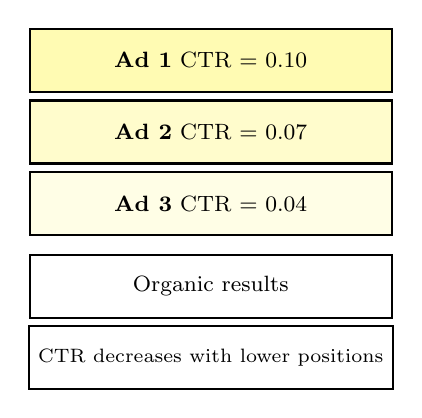
\begin{tikzpicture}[baseline=(current bounding box.north),scale=0.7, every node/.style={draw, thick, minimum height=0.8cm, align=left, font=\footnotesize}]
      \node[fill=yellow!30, minimum width=4.6cm, align=left] at (0,2.2) {\textbf{Ad 1} \hfill CTR = 0.10};
      \node[fill=yellow!20, minimum width=4.6cm, align=left] at (0,0.9) {\textbf{Ad 2} \hfill CTR = 0.07};
      \node[fill=yellow!10, minimum width=4.6cm, align=left] at (0,-0.4) {\textbf{Ad 3} \hfill CTR = 0.04};
      \node[draw, fill=white, minimum width=4.6cm, minimum height=0.8cm] at (0,-1.9) {Organic results};
      % small legend/annotation
      \node[anchor=north, font=\scriptsize] at (0,-2.6) {CTR decreases with lower positions};
    \end{tikzpicture}
\end{columns}

\vspace{0.8ex}
\textbf{Key Feature:} Click-through rate (CTR) decreases with position
\end{frame}

\begin{frame}{Position Auction Model}
\textbf{Setup:}
\begin{itemize}
  \item $k$ positions (slots) with CTRs: $\alpha_1 > \alpha_2 > \cdots > \alpha_k > 0$
  \item $n$ advertisers with values per click: $v_1, v_2, \ldots, v_n$
  \item Advertisers submit bids: $b_1, b_2, \ldots, b_n$
\end{itemize}

\textbf{Allocation Rule:}
\begin{itemize}
  \item Rank advertisers by bid: $b_{(1)} \geq b_{(2)} \geq \cdots \geq b_{(n)}$
  \item Assign positions by rank: highest bidder $\rightarrow$ position 1, etc.
  \item Top $k$ bidders get slots
\end{itemize}

\textbf{Payment Rule:} Multiple possibilities
\begin{enumerate}
  \item \textbf{First-price:} Pay own bid per click
  \item \textbf{Generalized Second-Price (GSP):} Pay next-highest bid per click
  \item \textbf{VCG:} Pay opportunity cost
\end{enumerate}
\end{frame}

\begin{frame}{Generalized Second-Price (GSP) Auction}
\textbf{Format (Used by Google):}
\begin{itemize}
  \item Rank by bid: Highest bidder gets top slot, etc.
  \item Payment: Pay \textbf{next-highest bid} per click
  \item Bidder in position $i$ pays $b_{(i+1)}$ per click
\end{itemize}

\textbf{Example:} 3 slots, 3 bidders
\begin{center}
\begin{tabular}{cccc}
\toprule
Bidder & Value/click & Bid & Position \\
\midrule
A & \$10 & \$7 & 1 (pays \$5/click) \\
B & \$8 & \$5 & 2 (pays \$3/click) \\
C & \$6 & \$3 & 3 (pays \$0/click) \\
\bottomrule
\end{tabular}
\end{center}

\textbf{Expected Payments:}
\begin{itemize}
  \item A: $\alpha_1 \times 5$
  \item B: $\alpha_2 \times 3$
  \item C: $\alpha_3 \times 0$
\end{itemize}
\end{frame}

\begin{frame}{GSP vs. Standard Second-Price}
\textbf{Similarity:} Both charge next-highest bid

\textbf{Key Difference:} GSP is \textbf{not} truthful!

\textbf{Why?} Winning a higher position affects your payment

\textbf{Example:} 2 positions, CTRs $\alpha_1 = 0.1$, $\alpha_2 = 0.05$

Bidder A with $v_A = 10$:
\begin{itemize}
  \item Others bid: $b_B = 8$, $b_C = 5$
  \item If A bids $b_A = 9$: Position 1, pay $8 \times 0.1 = 0.8$
  \item If A bids $b_A = 7$: Position 2, pay $5 \times 0.05 = 0.25$
  \item Utility if position 1: $10 \times 0.1 - 0.8 = 0.2$
  \item Utility if position 2: $10 \times 0.05 - 0.25 = 0.25$
  \item \textbf{Better to bid lower and get position 2!}
\end{itemize}

\textbf{Implication:} Bidding true value is \textbf{not} optimal
\end{frame}

\begin{frame}{Locally Envy-Free Equilibrium}
\textbf{Nash Equilibrium in GSP:}

\begin{block}{Definition}
A bid profile is a \textbf{locally envy-free equilibrium} if no bidder wants to move to an adjacent position at current prices.
\end{block}

\textbf{Conditions:} For bidder in position $i$:
\begin{align*}
\alpha_i(v_i - p_i) &\geq \alpha_{i-1}(v_i - p_{i-1}) \quad \text{(don't want higher)} \\
\alpha_i(v_i - p_i) &\geq \alpha_{i+1}(v_i - p_{i+1}) \quad \text{(don't want lower)}
\end{align*}

where $p_i$ is price per click for position $i$.

\textbf{Interpretation:}
\begin{itemize}
  \item Happy with current position given prices; No incentive to deviate to adjacent slot
  \item May still want to jump multiple positions; Many equilibria exist in GSP!
\end{itemize}
\end{frame}

\begin{frame}{VCG for Position Auctions}
\textbf{VCG Applied to Positions:}

\textbf{Allocation:} Same as GSP - rank by value; \textbf{Intuition:} Pay for displacing others downward

\textbf{Payment:} Bidder $i$ in position $j$ pays:
$$p_i^{VCG} = \sum_{k=j+1}^{n} (v_k - v_{k+1})(\alpha_{k-1} - \alpha_k)$$

\textbf{Example:} 2 positions, values $v_1 = 10, v_2 = 8, v_3 = 5$
\begin{itemize}
  \item CTRs: $\alpha_1 = 0.10, \alpha_2 = 0.05, \alpha_3 = 0$
  \item Bidder 1 in position 1:
  $$p_1 = (8-5)(0.10 - 0.05) + (5-0)(0.05 - 0) = 0.15 + 0.25 = 0.40$$
  \item Bidder 2 in position 2:
  $$p_2 = (5-0)(0.05 - 0) = 0.25$$
\end{itemize}

\textbf{Property:} Truthful bidding is dominant strategy!
\end{frame}

\begin{frame}{GSP vs. VCG: Revenue Comparison}
\textbf{Theorem (Edelman-Ostrovsky-Schwarz 2007):}

The truthful VCG equilibrium is also a \textbf{lowest-revenue} equilibrium of GSP.

\textbf{Implication:} GSP can generate higher revenue than VCG!

\textbf{Why?}
\begin{itemize}
  \item GSP has multiple equilibria
  \item Some equilibria have higher prices than VCG
  \item Advertisers may coordinate on high-price equilibrium
\end{itemize}

\textbf{Example:} With 2 positions and values $v_1 = 10, v_2 = 8$:
\begin{itemize}
  \item VCG: Bidder 1 pays based on $v_2$
  \item GSP equilibrium: Could have $b_1 = 9, b_2 = 7$
  \item GSP payment higher than VCG
\end{itemize}

\textbf{Google's Choice:} Uses GSP, not VCG
\begin{itemize}
  \item Simpler to explain; Higher revenue in practice
  \item Price discovery through dynamics
\end{itemize}
\end{frame}

\begin{frame}{Quality Scores in Practice}
\textbf{Reality:} Google doesn't just rank by bid!

\textbf{Quality Score:} Combines multiple factors
\begin{itemize}
  \item Expected click-through rate (CTR); Ad relevance to query
  \item Landing page quality; Historical account performance
\end{itemize}

\textbf{Effective Ranking:} By $b_i \times q_i$ (bid $\times$ quality)

\textbf{Benefits:}
\begin{enumerate}
  \item \textbf{User experience:} Show relevant ads
  \item \textbf{Platform revenue:} More clicks = more revenue
  \item \textbf{Efficiency:} High-value ads get prominent positions
  \item \textbf{Incentives:} Encourage advertisers to improve quality
\end{enumerate}

\textbf{Trade-off:}
\begin{itemize}
  \item More complex mechanism; Quality scores may be manipulated
  \item Less transparent to advertisers
\end{itemize}
\end{frame}

\begin{frame}{Position Auctions: Key Takeaways}
\textbf{GSP (Generalized Second-Price):}
\begin{itemize}
  \item \textcolor{red}{Not truthful} - strategic bidding required
  \item Multiple Nash equilibria
  \item Can generate higher revenue than VCG
  \item Simple and practical
  \item Used by Google, Bing, etc.
\end{itemize}

\textbf{VCG for Positions: (Not used in practice)}
\begin{itemize}
  \item \textcolor{green!70!black}{Truthful} - dominant strategy
  \item Unique equilibrium
  \item Lower revenue than GSP equilibria
  \item More complex payments
\end{itemize}

\textbf{Practical Considerations:}
\begin{itemize}
  \item Quality scores improve outcomes; Price discovery through repeated auctions
  \item Learning and dynamics matter; Simplicity valued over theoretical optimality
\end{itemize}
\end{frame}

\begin{frame}{Position Auctions: Mathematical Details}
\small
\begin{align*}
\text{Surplus}_i &= \alpha_j\,(v_i - p_j), \text{where } \alpha_j \text{ is CTR and }p_j\text{ is price/click}\\[4pt]
\text{GSP equilibrium (bidder }i\text{ in pos.\ }j):\quad
&\alpha_j(v_i - b_{j+1}) \ge \alpha_{j-1}(v_i - b_j),\\
&\alpha_j(v_i - b_{j+1}) \ge \alpha_{j+1}(v_i - b_{j+2})\\[4pt]
\Longrightarrow\quad
&b_{j+1} \le v_i - \frac{\alpha_{j-1}}{\alpha_j}\,(v_i - b_j), \\
&b_{j+1} \ge v_i - \frac{\alpha_{j+1}}{\alpha_j}\,(v_i - b_{j+2})
\end{align*}
\textbf{Remark:} Multiple bid vectors can satisfy these inequalities (many GSP equilibria).
\end{frame}

\begin{frame}{Other Position auction applications}
\textbf{1. Sponsored Search:}
\begin{itemize}
  \item Google Ads, Bing Ads
  \item \$200+ billion annually
\end{itemize}

\textbf{2. Social Media:}
\begin{itemize}
  \item Facebook/Instagram sponsored posts; LinkedIn promoted content
  \item Position = visibility in feed
\end{itemize}

\textbf{3. E-commerce:}
\begin{itemize}
  \item Amazon sponsored products; eBay promoted listings
  \item Position in search results
\end{itemize}

\textbf{4. Video Platforms:}
\begin{itemize}
  \item YouTube ads; Pre-roll, mid-roll positions
  \item Different values by position
\end{itemize}

\textbf{Common Theme:} Multiple "slots" with decreasing value
\end{frame}

\begin{frame}{Position Auctions: Summary Table}
\begin{center}
\small
\begin{tabular}{lcc}
\toprule
\textbf{Feature} & \textbf{GSP} & \textbf{VCG} \\
\midrule
Allocation & Rank by bid & Rank by value \\
Payment & Next-highest bid & Opportunity cost \\
Truthful & No & Yes \\
Equilibria & Multiple & Unique \\
Revenue & Higher & Lower \\
Complexity & Simple & Complex \\
Used by Google & Yes & No \\
Efficiency & Yes (in equilibrium) & Yes \\
\midrule
\textbf{Best for:} & Revenue \& Simplicity & Truth-telling \\
\bottomrule
\end{tabular}
\end{center}

\textbf{Industry Standard:} GSP with quality scores
\begin{itemize}
  \item Balances revenue, efficiency, and user experience
  \item Proven at massive scale (billions of auctions daily)
  \item Theory provides insights but practice differs
\end{itemize}
\end{frame}

\section{Combinatorial Auctions}

\begin{frame}{The Package Bidding Problem}
\textbf{Motivation:} Often bidders want combinations of items, not individual items

\textbf{Examples:}
\begin{itemize}
  \item \textbf{Spectrum licenses:} Adjacent frequencies worth more together
  \item \textbf{Airport slots:} Need landing + takeoff slot
  \item \textbf{Supply chains:} Raw materials + manufacturing capacity
  \item \textbf{Transportation:} Multiple routes forming network
\end{itemize}

\begin{center}
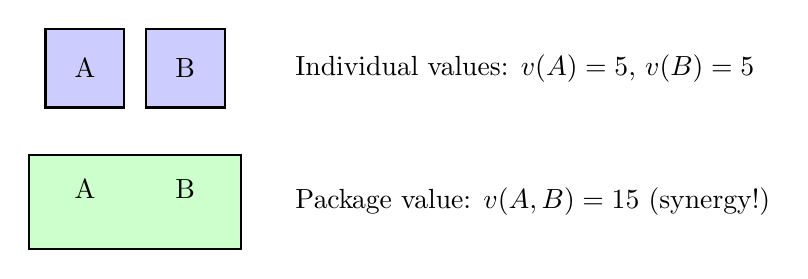
\begin{tikzpicture}[scale=0.85]
  % Individual items
  \node[draw, thick, fill=blue!20, minimum size=1cm] (A) at (0,0) {A};
  \node[draw, thick, fill=blue!20, minimum size=1cm] (B) at (1.5,0) {B};
  
  \node[right] at (3,0) {Individual values: $v(A) = 5$, $v(B) = 5$};
  
  % Package
  \node[draw, thick, fill=green!20, minimum width=2.7cm, minimum height=1.2cm] at (0.75,-2) {};
  \node at (0,-1.8) {A};
  \node at (1.5,-1.8) {B};
  
  \node[right] at (3,-2) {Package value: $v(A,B) = 15$ (synergy!)};
\end{tikzpicture}
\end{center}

\textbf{Key Issue:} $v(A \cup B) > v(A) + v(B)$ (complementarity)
\end{frame}

\begin{frame}[t]{Complementarity vs. Substitutability}
\small
\begin{columns}[t]
  \column{0.48\textwidth}
    \textbf{Complementarities:}\newline
    Value of bundle exceeds sum of parts
    \[
      v(S\cup T) > v(S) + v(T)
    \]
    \vspace{-0.5ex}
    \begin{itemize}\setlength\itemsep{0.5ex}
      \item Left shoe + Right shoe
      \item Adjacent spectrum licenses
      \item Hub airport + spoke airports
    \end{itemize}

  \column{0.48\textwidth}
    \textbf{Substitutes:}\newline
    Value of bundle less than sum of parts
    \[
      v(S\cup T) < v(S) + v(T)
    \]
    \vspace{-0.5ex}
    \begin{itemize}\setlength\itemsep{0.5ex}
      \item Two cars (only need one)
      \item Competing supply contracts
      \item Alternative shipping routes
    \end{itemize}
\end{columns}

\vspace{6ex}
\textbf{Challenge:} With $m$ items there are $2^m$ possible bundles --- e.g.\ 10 items = 1,024; 20 items = 1,048,576. Cannot simply ask for all values.
\end{frame}

\begin{frame}{Vickrey-Clarke-Groves: Efficient Truthful Bidding}
\begin{block}{Definition}
\small
The \textbf{VCG mechanism} (direct) asks bidders to report $v_i(S)$ for every bundle and then:
\[
S^*=\argmax_{\{S_i\}}\sum_i v_i(S_i)\quad\text{s.t. }S_i\cap S_j=\varnothing.
\]
Each winner pays the opportunity cost imposed on others:
\[
p_i=\max_{S_{-i}}\sum_{j\ne i}v_j(S_j)\;-\;\sum_{j\ne i}v_j(S_j^*),
\]
i.e., the value others would obtain without bidder $i$.
\end{block}

\textbf{Payment Interpretation:} Pay your \textbf{opportunity cost} imposed on others

\textbf{Key Property:} Truthful bidding is dominant strategy!
\end{frame}

\begin{frame}{VCG Example}
\textbf{Setup:} 2 items $\{A, B\}$, 2 bidders

\begin{center}
\begin{tabular}{l|cc|c}
\toprule
Bidder & $v(\{A\})$ & $v(\{B\})$ & $v(\{A,B\})$ \\
\midrule
1 & 5 & 5 & 15 \\
2 & 8 & 3 & 10 \\
\bottomrule
\end{tabular}
\end{center}

\textbf{Step 1: Efficient Allocation}
\begin{itemize}
  \item \textbf{Optimal:} Give both to 1, Value = 15
  \item Give A to 2, B to 1, Value = 8 + 5 = 13
  \item Give both to 2 Value = 10
\end{itemize}

\textbf{Step 2: VCG Payments}
\begin{itemize}
  \item Without 1: Best allocation is both to 2, value = 10
  \item With 1: Others (bidder 2) get nothing, value = 0
  \item \textbf{Bidder 1 pays:} $10 - 0 = 10$; \textbf{Bidder 2 pays:} 0 (didn't win)
\end{itemize}

\textbf{Outcome:} Bidder 1 gets $\{A,B\}$, surplus = $15 - 10 = 5$
\end{frame}

\begin{frame}{VCG, Why Truthful, proof sketch}
\begin{align*}
\text{Bidder } v_i \text{'s utility if reports } \hat{v}_i:\quad
& U_i = v_i(S_i^*) - p_i \\
\text{where } S_i^* \text{ is what } i \text{ gets, and}\quad
& p_i = \max_{S_{-i}} \sum_{j \neq i} v_j(S_j) - \sum_{j \neq i} v_j(S_j^*) \\
\text{Substituting:}\quad
& U_i = v_i(S_i^*) - \max_{S_{-i}} \sum_{j \neq i} v_j(S_j) + \sum_{j \neq i} v_j(S_j^*) \\
&= \underbrace{\left[v_i(S_i^*) + \sum_{j \neq i} v_j(S_j^*)\right]}_{\text{Total value with } i}
 - \underbrace{\max_{S_{-i}} \sum_{j \neq i} v_j(S_j)}_{\text{Constant (doesn't depend on } \hat{v}_i)}.
\end{align*}

\textbf{Key:} Maximizing $U_i$ is same as maximizing total value! Truth-telling achieves this maximum. $\square$
\end{frame}

\begin{frame}{VCG: Problems in Practice}
\textbf{Advantages:}
\begin{itemize}
  \item Efficient allocation; Dominant strategy incentive compatible; Individually rational
\end{itemize}

\textbf{Problems:}
\begin{enumerate}
  \item \textbf{Computational complexity:} NP-hard to find optimal allocation
  \begin{itemize}
    \item With $m$ items, need to solve over $2^m$ bundles
    \item Approximations may not preserve incentive properties
  \end{itemize}
  
  \item \textbf{Low revenue:} Can be arbitrarily low
  \begin{itemize}
    \item Revenue can be 0 even when values high!
    \item Not revenue maximizing
  \end{itemize}
  
  \item \textbf{Budget deficit:} $\sum_i p_i < 0$ possible
  \begin{itemize}
    \item May need to subsidize losing bidders
  \end{itemize}
  
  \item \textbf{Vulnerable to collusion:} False-name bids
  \begin{itemize}
    \item Single bidder submits multiple identities
  \end{itemize}
\end{enumerate}

\textbf{Practical use:} Limited to small-scale applications
\end{frame}

\begin{frame}{Simultaneous Ascending Auction (SAA)}
\textbf{FCC Spectrum Auction Design:}

\textbf{Format:}
\begin{itemize}
  \item Multiple rounds
  \item Each round: Bidders submit bids on individual items
  \item Prices increase based on demand
  \item Bidders can assemble packages dynamically
\end{itemize}

\textbf{Activity Rules:}
\begin{itemize}
  \item Must bid on certain \# of items each round
  \item "Use it or lose it" - maintains bidding rights
  \item Prevents gaming and waiting
\end{itemize}

\textbf{Stopping Rule:}
\begin{itemize}
  \item Auction ends when no new bids in a round
  \item Winners are current high bidders
  \item Pay own bids (first-price)
\end{itemize}
\end{frame}

\begin{frame}[t]{SAA: Advantages and Disadvantages}
\small
\begin{columns}[t]
  \column{0.50\textwidth}
    \vspace{0pt}
    \begin{itemize}\setlength\itemsep{0.6ex}
      \item \textbf{Price discovery:} bidders learn values through the process
      \item \textbf{Simple:} bid on individual items (computationally light)
      \item \textbf{Flexible:} can assemble packages dynamically
      \item \textbf{Proven:} raised \$100+ billion for US government
    \end{itemize}

  \column{0.50\textwidth}
    \vspace{0pt}
    \begin{itemize}\setlength\itemsep{0.6ex}
      \item \textbf{Exposure problem:} risk of winning only some
        \begin{itemize}\setlength\itemsep{0.3ex}
          \item e.g. bid on A+B, win A only (worth much less)
        \end{itemize}
      \item \textbf{Not truthful:} strategic bidding required
      \item \textbf{May be inefficient:} due to exposure and strategic play
      \item \textbf{Threshold problem:} small bidders struggle
    \end{itemize}
\end{columns}

\vspace{0.5ex}
\begin{block}{Example (Exposure)}
\small
Want \{A,B\} valued at 15; items worth 2 each individually. If you win A but not B you get value 2 — bidders often shade bids to avoid this risk.
\end{block}
\end{frame}

\begin{frame}{Combinatorial Clock Auction (UK 4G Auction, 2013)}
\textbf{Phase 1: Clock Phase}
\begin{itemize}
  \item Auctioneer announces prices for each item; Bidders indicate desired quantities at current prices
  \item Prices increase for over-demanded items; Continue until supply = demand
\end{itemize}

\textbf{Phase 2: Supplementary Bids}
\begin{itemize}
  \item Bidders submit additional package bids; Can bid on packages not available in clock phase
  \item Subject to activity constraints
\end{itemize}

\textbf{Phase 3: Winner Determination}
\begin{itemize}
  \item Find allocation maximizing total value; Use all bids from both phases
  \item Solve optimization problem
\end{itemize}

\textbf{Phase 4: Pricing (Core Selecting)}
\begin{itemize}
  \item Set prices in the "core" (coalition-proof); Minimize revenue subject to core constraints
\end{itemize}
\end{frame}

\begin{frame}{The Core in Combinatorial Auctions}
\begin{block}{Definition}
A set of prices is in the \textbf{core} if no coalition of bidders can profitably deviate by forming their own allocation.
\end{block}

\textbf{Formally:} Prices $(p_1, \ldots, p_n)$ are in core if:
$$\sum_{i \in C} (v_i(S_i^*) - p_i) \geq \max_{T} \sum_{i \in C} v_i(T_i) \quad \forall \text{ coalitions } C$$

\textbf{Interpretation:}
\begin{itemize}
  \item Winners cannot profitably block allocation and losers cannot outbid winners collectively, stability
\end{itemize}

\textbf{Core-Selecting Auctions:}
\begin{itemize}
  \item Choose prices in core that maximize revenue; More revenue than VCG (typically)
  \item Still efficient allocation; Used in modern spectrum auctions
\end{itemize}
\end{frame}

\begin{frame}{Combinatorial Auctions: Summary}
\begin{center}
\begin{tabular}{lccc}
\toprule
\textbf{Property} & \textbf{VCG} & \textbf{SAA} & \textbf{CCA} \\
\midrule
Efficient & Yes & No & Yes \\
Truthful & Yes & No & No \\
Revenue & Low & High & High \\
Computational & Hard & Easy & Hard \\
Exposure Risk & No & Yes & No \\
Price Discovery & No & Yes & Some \\
Used in Practice & Rare & Often & Growing \\
\bottomrule
\end{tabular}
\end{center}

\textbf{Trade-offs:}
\begin{itemize}
  \item Efficiency vs. Simplicity
  \item Truth-telling vs. Revenue
  \item Theory vs. Practice
\end{itemize}

\textbf{Current Trend:} Hybrid designs (CCA) combining advantages
\end{frame}

\section{Collusion in Auctions}

\begin{frame}{Collusion in Auctions}
\textbf{Definition:} Agreement among bidders to coordinate bids

\textbf{Why It Matters:}
\begin{itemize}
  \item Destroys competition
  \item Reduces seller revenue dramatically
  \item Illegal in most jurisdictions
  \item Difficult to detect and prevent
\end{itemize}

\textbf{Famous Examples:}
\begin{itemize}
  \item US school milk contracts (1980s-90s)
  \item Government procurement worldwide
  \item Art auctions (dealer rings)
  \item Spectrum auctions
\end{itemize}

\textbf{Key Question:} How do bidders sustain collusion?
\begin{itemize}
  \item Who should win?;How to split gains?;How to enforce agreement?
\end{itemize}
\end{frame}

\begin{frame}{Ring Formation}
\textbf{Cartel ("Ring") Problem:}
\begin{enumerate}
  \item Decide who bids in main auction
  \item Allocate object internally
  \item Distribute collusive surplus
\end{enumerate}

\textbf{Simple Model (Graham-Marshall 1987):}
\begin{itemize}
  \item $n$ ring members with values $v_1, \ldots, v_n$
  \item Designate bidder with highest value: $v_{(1)}$
  \item Only $v_{(1)}$ bids seriously in main auction
  \item Others submit low bids
  \item Winner pays approximately seller's reserve
\end{itemize}

\textbf{Surplus to Split:}
$$S = (v_{(1)} - r) - (v_{(1)} - v_{(2)}) = v_{(2)} - r$$

where $r$ is winning price (reserve or competitive bid from outside)

\textbf{Paradox:} Ring's surplus doesn't depend on $v_{(1)}$!
\end{frame}

\begin{frame}{Knockout Auctions}
\textbf{How to Allocate Internally:}
\begin{itemize}
  \item Pre-auction: Ring members hold "knockout" auction
  \item Winner of knockout bids in main auction
  \item Losers get side payments
\end{itemize}

\textbf{Common Formats:}
\begin{enumerate}
  \item \textbf{First-price knockout:}
  \begin{itemize}
    \item Ring members bid
    \item Highest bidder wins right to bid in main auction
    \item Pays bid to other ring members (split equally)
  \end{itemize}
  
  \item \textbf{Second-price knockout:}
  \begin{itemize}
    \item Highest bidder wins
    \item Pays second-highest bid to ring
  \end{itemize}
\end{enumerate}

\textbf{Key Insight:} Knockout auction induces truthful revelation among ring members!

\textbf{Evidence:} Found in antique auctions (Phillips report), procurement contracts
\end{frame}

\begin{frame}{Collusion Stability}
\textbf{Challenges to Maintaining Cartel:}

\textbf{1. Incentive to Deviate:}
\begin{itemize}
  \item Member might bid seriously to win directly
  \item Trade-off: Cheat gain vs. future collusion value
\end{itemize}

\textbf{2. Entry of Outsiders:}
\begin{itemize}
  \item New bidders break collusion
  \item Need to identify ring members (hard in sealed-bid)
\end{itemize}

\textbf{3. Enforcement:}
\begin{itemize}
  \item Illegal agreements unenforceable in court
  \item Rely on repeated game punishments
  \item Need to detect deviations
\end{itemize}

\textbf{Conditions for Stable Collusion:}
\begin{itemize}
  \item Small number of bidders (easier coordination); Frequent interactions (repeated game)
  \item Observable bids (detect deviations); Symmetric bidders (easier to agree)
\end{itemize}
\end{frame}

\begin{frame}{Optimal Auctions with Collusion}
\textbf{Seller's Response to Collusion Risk:}

\textbf{Marshall-Marx (2007) Results:}
\begin{enumerate}
  \item \textbf{Ascending auctions facilitate collusion}
  \begin{itemize}
    \item Information revelation helps coordination
    \item Easy to detect deviations
  \end{itemize}
  
  \item \textbf{Sealed-bid auctions hinder collusion}
  \begin{itemize}
    \item No information revelation; Hard to detect deviations
    \item Members uncertain about others' values
  \end{itemize}
  
  \item \textbf{Optimal response:}
  \begin{itemize}
    \item Use sealed-bid formats; Set high reserve prices
    \item Encourage entry of new bidders; Randomize auction procedures
  \end{itemize}
\end{enumerate}

\textbf{Revenue Ranking with Collusion Risk:}
$$\text{Sealed-bid} > \text{English (open ascending)}$$

\textit{Reverses standard ranking!}
\end{frame}

%===============================================


%===============================================
\part{Applications}
\partslide
\section{Real-World Examples}
%===============================================

\begin{frame}{Google Ads Auction}
\textbf{Generalized Second-Price (GSP):}
\begin{itemize}
  \item Multiple ad slots (positions)
  \item Bidders submit bids per click
  \item Allocation: Highest bids get top positions
  \item Payment: Pay next-highest bid
\end{itemize}

\textbf{Key Features:}
\begin{itemize}
  \item Billions of auctions daily
  \item Quality score adjusts effective bids
  \item Not fully truthful (strategic bidding remains)
  \item Revenue: \$200+ billion annually
\end{itemize}

\textbf{Design Challenge:}
\begin{itemize}
  \item Balance advertiser incentives with user experience
  \item Account for click-through rate differences
\end{itemize}
\end{frame}

\begin{frame}{Spectrum Auctions}
\textbf{FCC Spectrum Auctions:}
\begin{itemize}
  \item Multiple licenses (geography $\times$ frequency)
  \item Package bidding (combinatorial)
  \item Complex complementarity and substitution
  \item Stakes: \$100+ billion raised
\end{itemize}

\textbf{Design Evolution:}
\begin{itemize}
  \item 1994: Simultaneous ascending auction
  \item 2008: Package bidding introduced
  \item 2017: Incentive auction (buy back + resell)
\end{itemize}

\textbf{Lessons:}
\begin{itemize}
  \item Simple ascending works well for many items
  \item Activity rules prevent gaming
  \item Information revelation crucial
\end{itemize}
\end{frame}

\begin{frame}{Treasury Auctions}
\textbf{US Treasury Securities:}
\begin{itemize}
  \item Multiple units (billions of dollars)
  \item Discriminatory for bills
  \item Uniform for notes and bonds
  \item Annual volume: \$12+ trillion (2023)
\end{itemize}

\textbf{Why Different Formats?}
\begin{itemize}
  \item Bills: Short-term, simple valuation
  \item Notes/Bonds: Longer-term, more uncertainty
  \item Uniform reduces winner's curse for longer maturities
\end{itemize}

\textbf{Key Features:}
\begin{itemize}
  \item Non-competitive bids (small investors)
  \item Competitive bids (large institutions)
  \item Predictable schedule builds liquidity
\end{itemize}
\end{frame}

\begin{frame}{Online Marketplaces: eBay vs. Amazon}
\begin{center}
\begin{tabular}{p{4.5cm}p{4.5cm}}
\toprule
\textbf{eBay Model} & \textbf{Amazon Model} \\
\midrule
\rowcolor{blue!10}
English auction & Fixed price \\
\rowcolor{green!10}
Time-limited bidding & Immediate purchase \\
\rowcolor{blue!10}
Price discovery & Price transparency \\
\rowcolor{green!10}
Competition visible & Competition hidden \\
\rowcolor{blue!10}
Good for unique items & Good for commodities \\
\bottomrule
\end{tabular}
\end{center}

\textbf{Trend:} Even eBay emphasizes "Buy It Now" for speed

\textbf{Lesson:} Choose mechanism based on:
\begin{itemize}
  \item Product uniqueness
  \item Buyer urgency
  \item Transaction costs
\end{itemize}
\end{frame}

\section{Procurement}

\begin{frame}{Reverse Auctions for Procurement}
\textbf{Format:} Seller runs auction, buyers bid to supply

\textbf{Best Practices:}
\begin{itemize}
  \item \textbf{Qualify suppliers first:} Don't sacrifice quality for price
  \item \textbf{Clear specifications:} Avoid apples-to-oranges
  \item \textbf{Multiple rounds:} Give suppliers chance to compete
  \item \textbf{Reserve your right:} Don't have to accept lowest bid
\end{itemize}

\textbf{Common Mistakes:}
\begin{itemize}
  \item Running with only 2-3 suppliers
  \item Poorly defined requirements
  \item Focusing only on price, ignoring total cost
  \item Burning supplier relationships
\end{itemize}

\textbf{When to Avoid:}
\begin{itemize}
  \item Strategic partnerships; Highly customized products
  \item When you need innovation, not just low price
\end{itemize}
\end{frame}

\section{Marketplace Design}

\begin{frame}{Building a Marketplace: Two-Sided Markets}
\textbf{Your Platform Connects Buyers and Sellers}

Examples: eBay, Airbnb, Uber, AWS

\textbf{Key Challenges:}
\begin{itemize}
  \item \textbf{Chicken-and-egg:} Need both sides
  \item \textbf{Pricing:} Who pays? How much?
  \item \textbf{Quality:} How to maintain standards?
\end{itemize}

\textbf{Auction Design Helps:}
\begin{itemize}
  \item \textbf{Price discovery:} Market finds right price
  \item \textbf{Matching:} Right buyers find right sellers
  \item \textbf{Efficiency:} Resources to highest value use
\end{itemize}

\textbf{Critical Decision:} What's your objective?
\begin{itemize}
  \item Transaction volume? Revenue? Efficiency? Quality?
\end{itemize}
\end{frame}

\begin{frame}{Marketplace Design: Strategic Choices}
\begin{tabular}{|p{2.8cm}|p{3.4cm}|p{2.8cm}|}
\hline
\textbf{Choice} & \textbf{Option A} & \textbf{Option B} \\
\hline
\textbf{Pricing} & 
Commission &
Subscription/fees \\
\hline
\textbf{Competition} & 
Winner-take-all &
Multiple winners \\
\hline
\textbf{Transparency} & 
Show all bids &
Hide info \\
\hline
\textbf{Speed} & 
Real-time &
Batch at intervals \\
\hline
\textbf{Commitment} & 
Binding immediately &
Can cancel \\
\hline
\end{tabular}
\end{frame}

\section{Business Decision Framework}

\begin{frame}{When Should You Use Auction Design?}
\textbf{Good Fit When:}
\begin{itemize}
  \item Selling/buying scarce resources
  \item Value varies significantly across bidders
  \item You need price discovery
  \item You want competition to drive value
  \item You need transparent, defensible process
\end{itemize}

\textbf{Red Flags:}
\begin{itemize}
  \item Few potential bidders (collusion risk)
  \item High complexity (hard to participate)
  \item Unclear valuation (creates uncertainty)
  \item High transaction costs
\end{itemize}
\end{frame}

\begin{frame}{Decision Framework: 5 Key Questions}
\textbf{Before designing an auction:}

\begin{enumerate}
  \item \textbf{What are you selling?}
  \begin{itemize}
    \item Unique $\rightarrow$ English auction
    \item Commodity $\rightarrow$ Sealed-bid
  \end{itemize}
  
  \item \textbf{Who are your bidders?}
  \begin{itemize}
    \item Few sophisticated $\rightarrow$ Watch collusion
    \item Many casual $\rightarrow$ Keep simple
  \end{itemize}
  
  \item \textbf{What's your goal?}
  \begin{itemize}
    \item Max revenue $\rightarrow$ Set reserve
    \item Efficiency $\rightarrow$ English auction
  \end{itemize}
  
  \item \textbf{Time available?}
  \begin{itemize}
    \item Days/weeks $\rightarrow$ English
    \item Minutes/hours $\rightarrow$ Sealed-bid
  \end{itemize}
  
  \item \textbf{Risk tolerance?}
  \begin{itemize}
    \item Risk-averse $\rightarrow$ Higher reserve
    \item Risk-neutral $\rightarrow$ Optimize expected value
  \end{itemize}
\end{enumerate}
\end{frame}

\begin{frame}{Preventing Collusion}
\textbf{Warning Signs:}
\begin{itemize}
  \item Identical bids
  \item Rotating winners
  \item Intentionally low bids
  \item Few active bidders
\end{itemize}

\textbf{Countermeasures:}
\begin{itemize}
  \item Use sealed-bid formats; Set meaningful reserves
  \item Limit information disclosure; Random participation rules
  \item Prosecute violations; Encourage new entrants
\end{itemize}

\textbf{Best Practice:}
\begin{itemize}
  \item Monitor bidding patterns over time; Keep reserve prices confidential
  \item Use sealed formats when collusion risk high
\end{itemize}
\end{frame}

\begin{frame}{Implementation Checklist}
\textbf{Before Launching:}

\begin{enumerate}
  \item \textbf{Define Success Metrics}
  \begin{itemize}
    \item Revenue? Efficiency? Fairness? Speed?
  \end{itemize}
  
  \item \textbf{Know Your Participants}
  \begin{itemize}
    \item Sophistication and collusion potential
  \end{itemize}
  
  \item \textbf{Set Clear Rules}
  \begin{itemize}
    \item Reserve prices, activity requirements, payment
  \end{itemize}
  
  \item \textbf{Plan for Edge Cases}
  \begin{itemize}
    \item No bids? Same bids? Manipulation?
  \end{itemize}
  
  \item \textbf{Test and Monitor}
  \begin{itemize}
    \item Start small, gather data, iterate
  \end{itemize}
\end{enumerate}
\end{frame}

\begin{frame}{Red Flags: When Market Design Is Failing}
\textbf{Warning Signs:}
\begin{itemize}
  \item \textbf{Low participation:} Few bidders showing up
  \item \textbf{Unusual patterns:} Everyone bids same or very high/low
  \item \textbf{Complaints:} Rules unclear or unfair
  \item \textbf{Gaming:} Evidence of manipulation
  \item \textbf{Instability:} Prices swing wildly
  \item \textbf{Inefficiency:} Wrong winners
\end{itemize}

\textbf{What to Do:}
\begin{itemize}
  \item Don't ignore signals
  \item Gather data and analyze
  \item Consult participants
  \item Be willing to redesign
  \item Test changes carefully
\end{itemize}

\textit{California ignored warnings for months before crisis hit}
\end{frame}

%===============================================
\part{Double Auctions}
\partslide
%===============================================

\begin{frame}{Double Auctions: Definition}
\begin{block}{Definition}
A \textbf{double auction} is a mechanism where both buyers and sellers submit bids simultaneously. Trades occur when buy bids meet or exceed sell offers.
\end{block}

\textbf{Key Difference from Standard Auctions:}
\begin{itemize}
\item Standard: One seller, multiple buyers (or vice versa)
\item Double: Multiple buyers AND multiple sellers
\item Both sides strategic
\end{itemize}

\textbf{Applications:}
\begin{itemize}
  \item Stock exchanges (NYSE, NASDAQ); Commodity markets; Electricity markets
  \item Carbon emission trading; Decentralized prediction markets
\end{itemize}

\textbf{Question:} How to match buyers and sellers efficiently?
\end{frame}

\begin{frame}{Double Auction Setup}
\textbf{Players:}
\begin{itemize}
  \item $m$ buyers with private valuations $v_1, \ldots, v_m$
  \item $n$ sellers with private costs $c_1, \ldots, c_n$
  \item Values and costs drawn from distributions $F_v$ and $F_c$
\end{itemize}

\textbf{Actions:}
\begin{itemize}
  \item Buyer $i$ submits bid $b_i \leq v_i$
  \item Seller $j$ submits ask $a_j \geq c_j$
\end{itemize}

\textbf{Efficient Allocation:}
\begin{itemize}
  \item Order bids: $b_{(1)} \geq b_{(2)} \geq \cdots \geq b_{(m)}$
  \item Order asks: $a_{(1)} \leq a_{(2)} \leq \cdots \leq a_{(n)}$
  \item Trade quantity: $k^* = \max\{k : b_{(k)} \geq a_{(k)}\}$
  \item Gains from trade: $\sum_{i=1}^{k^*}(v_{(i)} - c_{(i)})$
\end{itemize}
\end{frame}

\begin{frame}{The $k$-Double Auction Rule}
\textbf{Trading Rule:} If buyer $i$ and seller $j$ are matched:
\begin{itemize}
  \item Trade occurs if $b_i \geq a_j$
  \item Trade price: $p = k \cdot b_i + (1-k) \cdot a_j$ where $k \in [0,1]$
\end{itemize}

\textbf{Special Cases:}
\begin{itemize}
  \item $k=0$: Buyer-bid auction (buyer pays bid, seller gets bid)
  \item $k=1$: Seller-ask auction (buyer pays ask, seller gets ask)
  \item $k=\frac{1}{2}$: Split-the-difference (average of bid and ask)
\end{itemize}

\textbf{Strategic Implications:}
\begin{itemize}
  \item $k=0$: Buyers bid like first-price auction (shade bids)
  \item $k=1$: Sellers bid like first-price auction (inflate asks)
  \item $k=\frac{1}{2}$: Both sides shade symmetrically
  \item No $k$ makes truthful bidding dominant for both sides!
\end{itemize}
\end{frame}

\begin{frame}{General Equilibrium Derivation}
\begin{align*}
b &\geq a(c);&& \\ 
p &= kb + (1-k)a(c);&&  \text{becomes} \quad kb + (1-k)b = b; \\
U_B(b|v) &= \Pr(\text{trade}) \cdot (v - p);&&  \\
U_B(b|v) &= F_c(a^{-1}(b)) \cdot (v - b);&&  \text{Using p=b} \\
\frac{f_c(v)}{a'(v)}& \cdot [v - b(v)] = F_c(v);&& b = b(v); \text{FOC and equilibrium} \\ 
\frac{f_v(c)}{b'(c)}& \cdot [a(c) - c] = 1 - F_v(c);&& \text{symmetrically for seller}
\end{align*}
\textbf{Result:} Coupled ODEs determining $b(v)$ and $a(c)$. 
\end{frame}

\begin{frame}{Equilibrium Bidding: Uniform Distribution}
\textbf{Setup:} One buyer with $v \sim U[0,1]$, one seller with $c \sim U[0,1]$

\textbf{Equilibrium Strategies (Chatterjee-Samuelson 1983):}
\begin{align*}
\text{Buyer bids:} \quad b(v) &= kv + \frac{1-k}{2} \\
\text{Seller asks:} \quad a(c) &= (1-k)c + \frac{k}{2}
\end{align*}

\textbf{Examples:}
\begin{center}
\begin{tabular}{cccc}
\toprule
$k$ & Buyer Bid $b(v)$ & Seller Ask $a(c)$ & Trade Price \\
\midrule
$0$ & $\frac{1}{2}$ & $c$ & $a(c) = c$ \\[0.2cm]
$\frac{1}{2}$ & $\frac{2v+1}{4}$ & $\frac{2c+1}{4}$ & $\frac{v+c+1}{4}$ \\[0.2cm]
$1$ & $v$ & $\frac{1}{2}$ & $b(v) = v$ \\
\bottomrule
\end{tabular}
\end{center}

\textbf{Key Insight:} Both sides shade away from truthful reporting
\end{frame}

\begin{frame}{Equilibrium Visualization: $k=0$ (Buyer-Bid Auction)}
\begin{center}
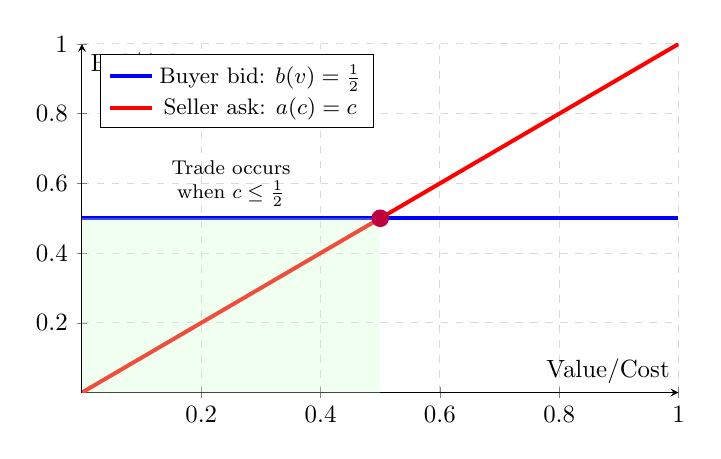
\begin{tikzpicture}[scale=0.9]
  \begin{axis}[
    xlabel={Value/Cost},
    ylabel={Bid/Ask},
    xmin=0, xmax=1,
    ymin=0, ymax=1,
    axis lines=middle,
    legend pos=north west,
    legend style={font=\small},
    width=10cm,
    height=6.5cm,
    grid=major,
    grid style={dashed, gray!30}
  ]
  
  % Buyer's bid (constant at 1/2)
  \addplot[domain=0:1, ultra thick, blue] {0.5};
  \addlegendentry{Buyer bid: $b(v) = \frac{1}{2}$}
  
  % Seller's ask (45-degree line)
  \addplot[domain=0:1, ultra thick, red] {x};
  \addlegendentry{Seller ask: $a(c) = c$}
  
  % Trade region
  \fill[green!20, opacity=0.3] (0,0) rectangle (0.5,0.5);
  \node[align=center, font=\footnotesize] at (0.25,0.60) {Trade occurs\\when $c \leq \frac{1}{2}$};
  
  % Intersection point
  \node[circle, fill=purple, inner sep=2.5pt] at (0.5,0.5) {};
  
  \end{axis}
\end{tikzpicture}
\end{center}

\textbf{Note:} Buyer always bids $\frac{1}{2}$, seller truthfully reveals cost
\end{frame}

\begin{frame}{Equilibrium Visualization: $k=\frac{1}{2}$ (Split-the-Difference)}
\begin{center}
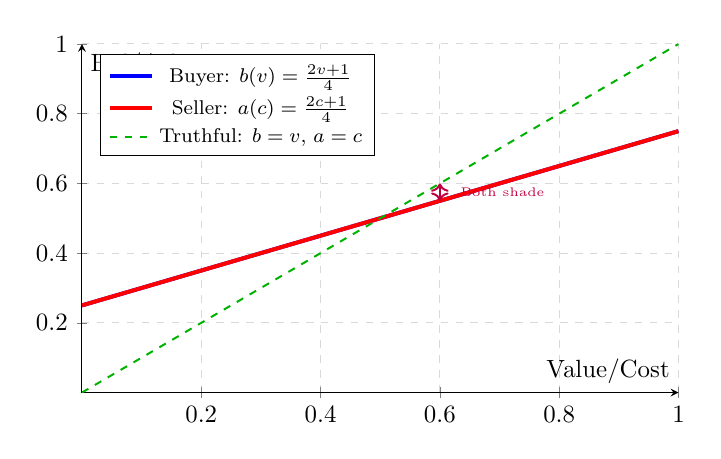
\begin{tikzpicture}[scale=0.9]
  \begin{axis}[
    xlabel={Value/Cost},
    ylabel={Bid/Ask},
    xmin=0, xmax=1,
    ymin=0, ymax=1,
    axis lines=middle,
    legend pos=north west,
    legend style={font=\footnotesize},
    width=10cm,
    height=6.5cm,
    grid=major,
    grid style={dashed, gray!30}
  ]
  
  % Buyer's bid
  \addplot[domain=0:1, ultra thick, blue] {0.5*x + 0.25};
  \addlegendentry{Buyer: $b(v) = \frac{2v+1}{4}$}
  
  % Seller's ask
  \addplot[domain=0:1, ultra thick, red] {0.5*x + 0.25};
  \addlegendentry{Seller: $a(c) = \frac{2c+1}{4}$}
  
  % Truthful bidding
  \addplot[domain=0:1, thick, dashed, green!70!black] {x};
  \addlegendentry{Truthful: $b=v$, $a=c$}
  
  % Annotations
  \draw[<->, thick, purple] (0.6,0.6) -- (0.6,0.55);
  \node[right, purple, font=\tiny] at (0.62,0.575) {Both shade};
  
  \end{axis}
\end{tikzpicture}
\end{center}

\textbf{Note:} Symmetric shading - both buyer and seller use same strategy function
\end{frame}

\begin{frame}{Equilibrium Visualization: $k=1$ (Seller-Ask Auction)}
\begin{center}
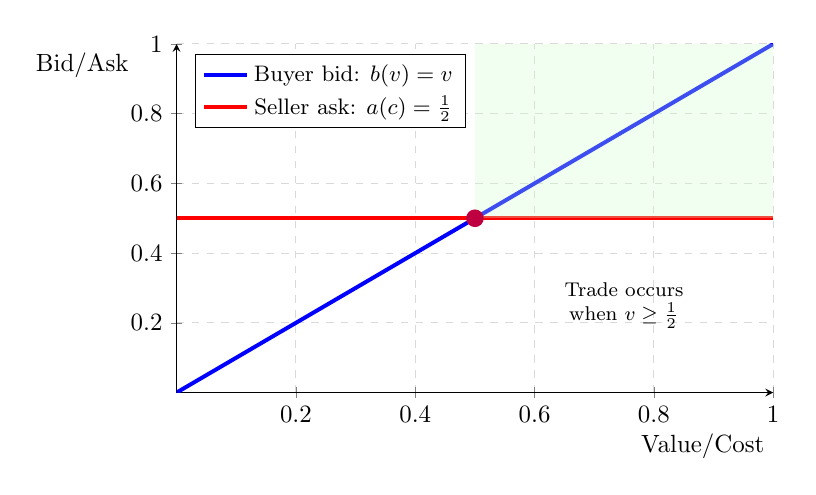
\begin{tikzpicture}[scale=0.9]
  \begin{axis}[
    xlabel={Value/Cost},
    ylabel={Bid/Ask},
    xmin=0, xmax=1,
    ymin=0, ymax=1,
    axis lines=middle,
    legend pos=north west,
    legend style={font=\small},
    width=10cm,
    height=6.5cm,
    xlabel style= {yshift=-30pt},
    ylabel style= {xshift=-60pt},
    grid=major,
    grid style={dashed, gray!30}
  ]
  
  % Buyer's bid (45-degree line)
  \addplot[domain=0:1, ultra thick, blue] {x};
  \addlegendentry{Buyer bid: $b(v) = v$}
  
  % Seller's ask (constant at 1/2)
  \addplot[domain=0:1, ultra thick, red] {0.5};
  \addlegendentry{Seller ask: $a(c) = \frac{1}{2}$}
  
  % Trade region
  \fill[green!20, opacity=0.3] (0.5,0.5) rectangle (1,1);
  \node[align=center, font=\footnotesize] at (0.75,0.25) {Trade occurs\\when $v \geq \frac{1}{2}$};
  
  % Intersection point
  \node[circle, fill=purple, inner sep=2.5pt] at (0.5,0.5) {};
  
  \end{axis}
\end{tikzpicture}
\end{center}

\textbf{Note:} Seller always asks $\frac{1}{2}$, buyer truthfully reveals value
\end{frame}

\begin{frame}{Double Auction: Key Results}
\begin{theorem}[Chatterjee-Samuelson 1983]
For the $k$-double auction with one buyer and one seller:
\begin{itemize}
  \item No $k \in [0,1]$ achieves ex-post efficiency; $k = \frac{1}{2}$ maximizes ex-ante gains from trade
  \item Equilibrium involves strategic misrepresentation by both sides
\end{itemize}
\end{theorem}

\begin{tcolorbox}[colback=blue!5!white,colframe=blue!75!black,title=Myerson-Satterthwaite Impossibility (1983)]
\textbf{No} mechanism can simultaneously achieve:
\begin{enumerate}
  \item Ex-post efficiency (trade whenever $v > c$)
  \item Individual rationality (voluntary participation)
  \item Balanced budget (no external subsidies)
  \item Incentive compatibility (truthful reporting)
\end{enumerate}
\end{tcolorbox}
\end{frame}

\begin{frame}{Efficiency with Many Traders}
\begin{center}
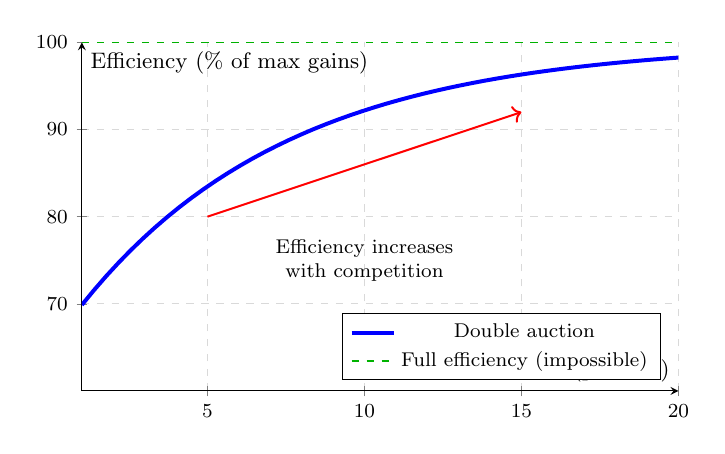
\begin{tikzpicture}[scale=0.9]
  \begin{axis}[
    xlabel={Number of Traders (per side)},
    ylabel={Efficiency (\% of max gains)},
    xmin=1, xmax=20,
    ymin=60, ymax=100,
    axis lines=middle,
    width=10cm,
    height=6.5cm,
    grid=major,
    grid style={dashed, gray!30},
    xtick={1,5,10,15,20},
    ytick={60,70,80,90,100},
    xlabel style={font=\small},
    ylabel style={font=\small},
    tick label style={font=\footnotesize},
    legend pos=south east,
    legend style={font=\footnotesize}
  ]
  
  % Efficiency curve
  \addplot[domain=1:20, samples=50, ultra thick, blue] {100 - 35*exp(-0.15*x)};
  \addlegendentry{Double auction}
  
  % 100% efficiency line
  \addplot[domain=1:20, samples=2, thick, dashed, green!70!black] {100};
  \addlegendentry{Full efficiency (impossible)}
  
  % Annotations
  \node[align=center, font=\footnotesize] at (axis cs:10,75) {Efficiency increases\\with competition};
  
  \draw[->, thick, red] (axis cs:5,80) -- (axis cs:15,92);
  
  \end{axis}
\end{tikzpicture}
\end{center}

\textbf{Key Insight:} With many traders (e.g., 10+ per side), double auctions achieve near-perfect efficiency despite strategic behavior (Gresik-Satterthwaite 1989)
\end{frame}


%===============================================
\part{Summary}
\partslide
\section{Key Takeaways}
%===============================================

\begin{frame}{Summary: Core Results}
\textbf{1. Equilibrium Strategies:}
\begin{itemize}
  \item English/Vickrey: Bid true value (dominant)
  \item First-Price/Dutch: Shade bid below value
  \item All-Pay: Much more conservative bidding
\end{itemize}

\textbf{2. Revenue Equivalence (IPV, risk-neutral, symmetric):}
\begin{itemize}
  \item All standard formats yield same revenue
  \item Revenue = $\E[v_{(2)}]$
  \item Breaks with risk aversion, asymmetry, or correlation
\end{itemize}

\textbf{3. Optimal Design:}
\begin{itemize}
  \item Reserve price improves revenue
  \item Virtual valuation determines optimal allocation
  \item Information revelation increases revenue with affiliation
\end{itemize}
\end{frame}

\begin{frame}{Summary: Bid Functions (Uniform Distribution)}
\begin{center}
\begin{tabular}{lcc}
\toprule
\textbf{Format} & \textbf{Equilibrium Bid} $B(v)$ & \textbf{Revenue} \\
\midrule
English & $v$ & $\frac{n-1}{n+1}$ \\[0.2cm]
Second-Price & $v$ & $\frac{n-1}{n+1}$ \\[0.2cm]
First-Price & $\frac{n-1}{n}v$ & $\frac{n-1}{n+1}$ \\[0.2cm]
Dutch & $\frac{n-1}{n}v$ & $\frac{n-1}{n+1}$ \\[0.2cm]
All-Pay 1st & $\frac{n-1}{n}v^n$ & $\frac{n-1}{n+1}$ \\[0.2cm]
War of Attrition & $v + (1-v)\ln(1-v)$ & $\frac{n-1}{n+1}$ \\
& (for $n=2$) & \\
\bottomrule
\end{tabular}
\end{center}

\textbf{Key:} Revenue Equivalence holds under benchmark assumptions
\end{frame}

\begin{frame}{Practical Guidelines}
\begin{tcolorbox}[colback=green!5,colframe=green!40!black,title=DO]
\begin{itemize}
  \item Set a reserve price (almost always)
  \item Monitor for collusion patterns and use sealed bids when collusion risk high
  \item Keep rules simple and transparent
  \item Reveal information with affiliated values
\end{itemize}
\end{tcolorbox}

\begin{tcolorbox}[colback=red!5,colframe=red!40!black,title=DON'T]
\begin{itemize}
  \item Assume revenue equivalence always holds
  \item Reveal sensitive competitive information
  \item Use complex formats without expert help
  \item Ignore entry barriers and participation costs
\end{itemize}
\end{tcolorbox}
\end{frame}

\begin{frame}{Key Takeaways for Business}
\textbf{The Big Ideas:}

\begin{enumerate}
  \item \textbf{Design matters more than theory}
  \begin{itemize}
    \item Real-world context beats textbook
  \end{itemize}
  
  \item \textbf{Auctions reveal private information}
  \begin{itemize}
    \item Better than posted prices when values uncertain
  \end{itemize}
  
  \item \textbf{Format choice depends on context}
  \begin{itemize}
    \item Under ideal conditions, all yield same revenue
    \item Choose based on practical considerations
  \end{itemize}
  
  \item \textbf{Real markets violate assumptions}
  \begin{itemize}
    \item Risk aversion, collusion, entry costs matter
  \end{itemize}
  
  \item \textbf{Simplicity beats sophistication}
  \begin{itemize}
    \item Participants must understand mechanism
  \end{itemize}
\end{enumerate}
\end{frame}


\begin{frame}{Additional Resources}
\textbf{Books:}
\begin{itemize}
  \item "Auction Theory" by Vijay Krishna (intermediate)
  \item "Putting Auction Theory to Work" by Paul Milgrom (advanced)
\end{itemize}

\textbf{Industry Examples:}
\begin{itemize}
  \item FCC Spectrum Auctions (www.fcc.gov/auctions)
  \item Treasury Securities (www.treasurydirect.gov)
  \item Google Ads Help Center
\end{itemize}

\textbf{Expert Consultants:}
\begin{itemize}
  \item For high-stakes auctions (>\$1M)
  \item Firms: NERA, Compass Lexecon, Analysis Group
\end{itemize}

\begin{center}
\Large Questions?
\end{center}
\end{frame}

\end{document}
